\documentclass{beamer}
\usetheme{metropolis}
\usepackage{lmodern}
\author{Ravshanbek Khodzhimatov \\Thesis Advisor: Assoc. Prof. Dr. Tolga Umut Kuzuba\c{s}}
\title{Welfare Comparison of Different Life-Cycle Investment Strategies for Turkey}
\subtitle{Master's Thesis}
\usepackage{amsmath}
\usepackage{booktabs}
\usepackage{graphicx}
\usepackage{amsfonts}
\usepackage{geometry}
\usepackage{nameref}
\usepackage{tikz}
\beamertemplatenavigationsymbolsempty


%%%%%%%%%%%%%%%%%%%%%%%%%%%%%%%%%%
\begin{document}

\begin{frame}
\titlepage
\end{frame}

\section{Introduction}

\begin{frame}[allowframebreaks]{Introduction}
  \begin{itemize}
	\item Retirement is one of the most important investment decisions we face in our lives.
	\item Current investment menus are either too simplistic and inefficient or too complicated and unintuitive.
	\item Most individuals find active involvement in investment too complex.
	\item Lifecycle investments --- investments that are designed for different age profiles, as opposed to fixed-over-lifetime investments.
	\item Naive investments --- asset allocations that do not consider individual characteristics. 

\framebreak

\begin{table}
	\centering
	\caption{Largest Turkish Pension Funds}
	\begin{tabular}[H]{lc}
		\hline
		Fund name&Fund size\\
		\hline
		AvivaSA Emeklilik ve Hayat&14.8 bln\\
		Anadolu Hayat Emeklilik&14.1 bln\\
		Garanti Emeklilik ve Hayat&11.1 bln\\
		Allianz Yasam ve Emeklilik&10.4 bln\\
		Vakif Emeklilik&6.1 bln\\
		\hline
	\end{tabular}\\
	Source: Pension Monitoring Center (2018)
\end{table}
	
  \end{itemize}
\end{frame}


\section{Literature Review}

\begin{frame}[allowframebreaks]{Literature Review}
  \begin{itemize}
	\item Markowitz's Mean-Variance Analysis --- maximize return while minimizing volatility:
\begin{center}
  $\displaystyle\max_{\alpha} \{ E[R_p] - \frac{\gamma}{2}\sigma^2_p \}$
\end{center}
solution:
\begin{center}
	$\alpha = \frac{E[R] - R_f}{\gamma\sigma^2}$
\end{center}
where $\alpha$ is risky asset share in portfolio.

	\item Markowitz derived fixed one-period solution.

\framebreak
	
	\item Merton (1971) generalized the problem to multiple periods, found it optimal to repeat Markowitz every period.
	
	\item Contradicted financial advice and rationality $\alpha_t = (100-t)\%$

	\item Bodie (1992) added human capital (discounted sum of future fixed wage) into the model:
  
\begin{center}
	$\alpha_t = \frac{\mu - R_f}{\gamma \sigma^2}\left(1+\frac{L_t}{F_t}\right)$
\end{center}

	\item $L_t/F_t$ changed over time and captured lifecycle effect. Young people would be more aggressive than Markowitz, and old people would converge to Markowitz.

\framebreak
	
	\item Cocco et al. (2005) did similar analysis and added the following heuristic:


\begin{center}
	$\alpha_t = \begin{cases} 100\% & t<40\\(200-2.5t)\% & t\in[40,60]\\50\% & t>60 \end{cases}$,
\end{center}

	\item Did not explain hump-shaped stock share (Chang (2014))
	\begin{center}
		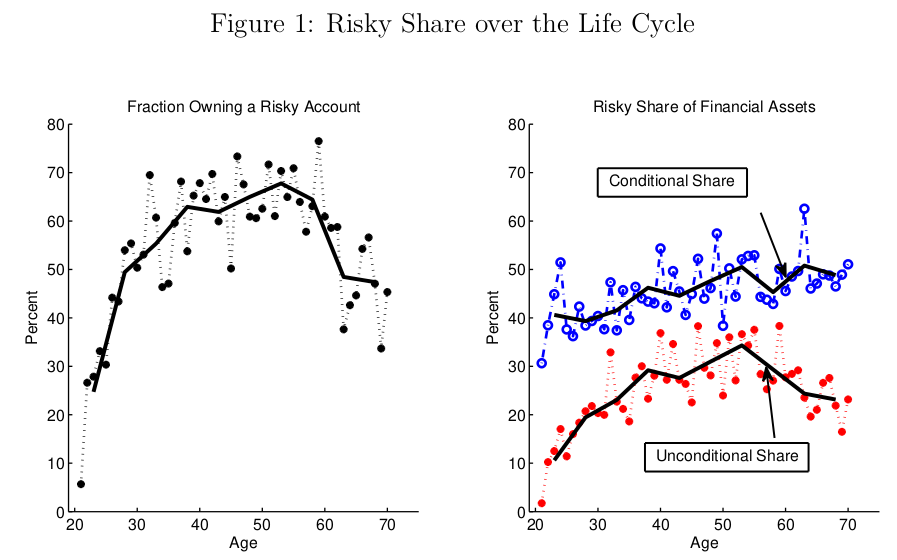
\includegraphics[scale=0.3]{figs/chang.png}
	\end{center}
	\item Cocco and Flavin and Yamashita (2002) found that if individuals possessed housing, they would be even more aggressive, using dynamic optimization.

\framebreak

	\item Munk (2016) reinvented analytical solution to the problem.

\begin{center}
	$ \displaystyle\max_{\pi} \{ E[\frac{W_1}{W_0}] - \frac{\gamma}{2} var(\frac{W_1}{W_0}) \} $
\end{center}

where total wealth is a sum of financial and human wealth: $W_t = F_t + L_t$ and human capital has returns $r_L \sim (\mu_L, \sigma_L)$.

\begin{center}
	$\pi^* = \frac{1}{\gamma} \frac{W_0}{F_0} \cdot \Sigma^{-1} (\mu - r_f \cdot 1) - \frac{L_0}{F_0} \cdot \Sigma^{-1} cov(r,r_L)$
\end{center}

\framebreak

	\item We used Munk's solution without housing:

\begin{center}
	$\pi_{t+1} = \frac{\mu_s - r_f}{\gamma \sigma^2_s}  + \frac{L_t}{F_t} \cdot \left(\frac{\mu_s - r_f}{\gamma \sigma^2_s} - \frac{\rho_{SL}\sigma_L}{\sigma_S} \right)$
\end{center}

	and with housing:

\begin{center}
	$\pi_{t+1} = \frac{1}{\gamma (1 - \rho^2_{SH}) \sigma_S} \cdot \frac{W_t}{F_t} \left( \frac{\mu_s - r_f}{\sigma_S} - \rho_{SH} \frac{\mu_h - r_f}{\sigma_h} \right) - \frac{L_t}{F_t} \cdot \frac{\sigma_L}{\sigma_S} \frac{\rho_{SL} - \rho_{SH}\rho_{HL}}{1 - \rho^2_{SH}}$
\end{center}
\begin{center}
	$\pi_{h,t+1} = \frac{1}{\gamma (1 - \rho^2_{SH}) \sigma_H} \cdot \frac{W_t}{F_t} \left( \frac{\mu_h - r_f}{\sigma_h} - \rho_{SH} \frac{\mu_s - r_f}{\sigma_s} \right) - \frac{L_t}{F_t} \cdot \frac{\sigma_L}{\sigma_h} \frac{\rho_{HL} - \rho_{SH}\rho_{SL}}{1 - \rho^2_{SH}}$
\end{center}
\begin{center}
	$\pi_{R_f} = \left( 1 - \pi - \pi_h \right)$
\end{center}

  \end{itemize}
\end{frame}

\section{Model}

\begin{frame}[allowframebreaks]{Model}
  \begin{itemize}
	\item We use Olear's (2016) approach to model labor income:

\begin{center}
	$Y_{i,t+1} = 
	\begin{cases}
		Y_{it} (1 + g_{i,t+1} + \xi_t + \omega_{it}), & t \leq T \\
		\lambda (1 + f(T, Z_{iT}) + v_{iT}), & t > T
	\end{cases}	
	$
\end{center}

	\item We model labor income, house prices, and stock prices as Geometric Brownian Motions with drifts $\mu_L$, $\mu_H$, $\mu_S$ and volatilities $\sigma_L$, $\sigma_H$, $\sigma_S$,
%	\item We model two risky assets and a wage as correlated discrete series:\\
%$\frac{\Delta S_{t+1}}{S_t} = \mu_s + \sigma_s \cdot \epsilon_{st}$\\
%$\frac{\Delta H_{t+1}}{H_t} = \mu_h + \sigma_h \cdot \left(\rho_{hs}\epsilon_{st} + (\sqrt{1-\rho^2_{hs}})\epsilon_{ht}\right)$\\
%$\frac{\Delta Y_{t+1}}{Y_t} = \mu_v + \sigma_v \cdot \left(\rho_{ys}\epsilon_{st} + \left(\frac{\rho_{yh} - \rho_{sh}\rho_{sy}}{\sqrt{1-\rho^2_{sh}}}\right)\epsilon_{ht} + \left(\sqrt{1-\rho^2_{ys}-(\frac{\rho_{yh} - \rho_{sh}\rho_{sy}}{\sqrt{1-\rho^2_{sh}}})^2}\right)\epsilon_{vt}\right)$

\framebreak

	\item Welfare measurement --- we use CRRA utility:

\begin{center}
$	E_1[U(c)] = \displaystyle\sum^T_{t=1} \delta^{t-1} \displaystyle\prod^{t-1}_{j=0} p_j \cdot \frac{c^{1-\gamma}_{it}}{1-\gamma}$
\end{center}

where $p_k$ is the probability of survival from time $k-1$ to time $k$.

	\item We omitted the bequest motives from the original formulation, thus retired person consumes all of his income at any given time.


\framebreak
	
	\item Retirement income --- accumulated financial wealth is repaid back in annuities.
	\item Reverse mortgages --- housing wealth is reinvested for annuities in return of inheriting a house to the payer (no bequest motives) 

\begin{center}
$	W_{65} = H_{65} + MP$
\end{center}

	\item Annuity is equal to:
$	A_t = W_{65} \cdot \left(1+\sum^{100}_{t=66} \frac{\prod^{t}_{j=66} p_j }{(1+r_f)^{t-65}} \right)^{-1}$	
	\item Welfare calculation --- we convert annuity stream into consumption (considering the inflation) and plug into CRRA expected utility function.

  \end{itemize}
\end{frame}

\section{Data Structure and Sources}

\begin{frame}[allowframebreaks]{Data Structure and Sources}
  \begin{itemize}

	\item Stock rates of return are obtained from Borsa Istanbul BIST30 index:

\begin{figure}
	\centering
	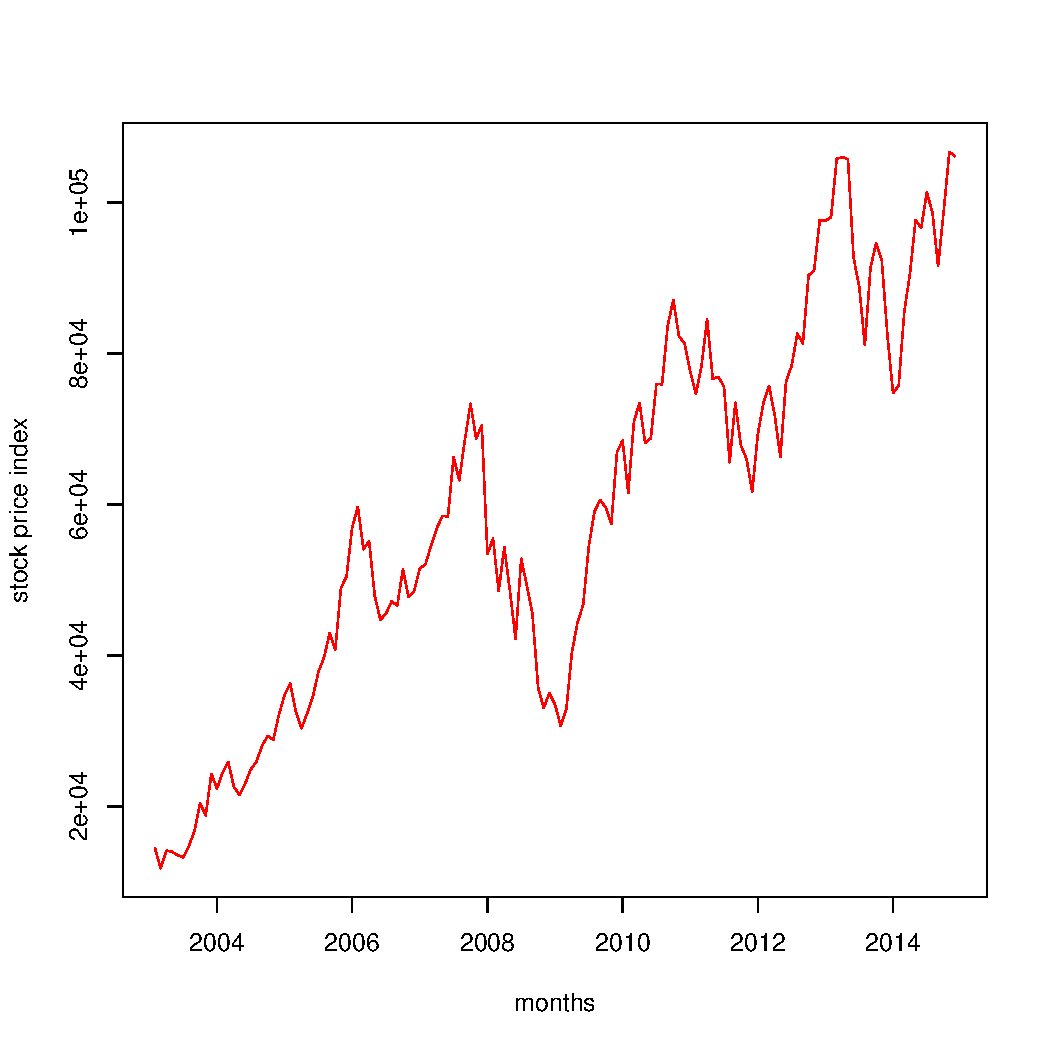
\includegraphics[scale=0.25]{figs/bist.pdf}
	\caption{BIST30 Turkish stock market performance index}
\end{figure}

\framebreak


	\item Housing returns are obtained from Reidin AEINDEXF index:

\begin{figure}
	\centering
		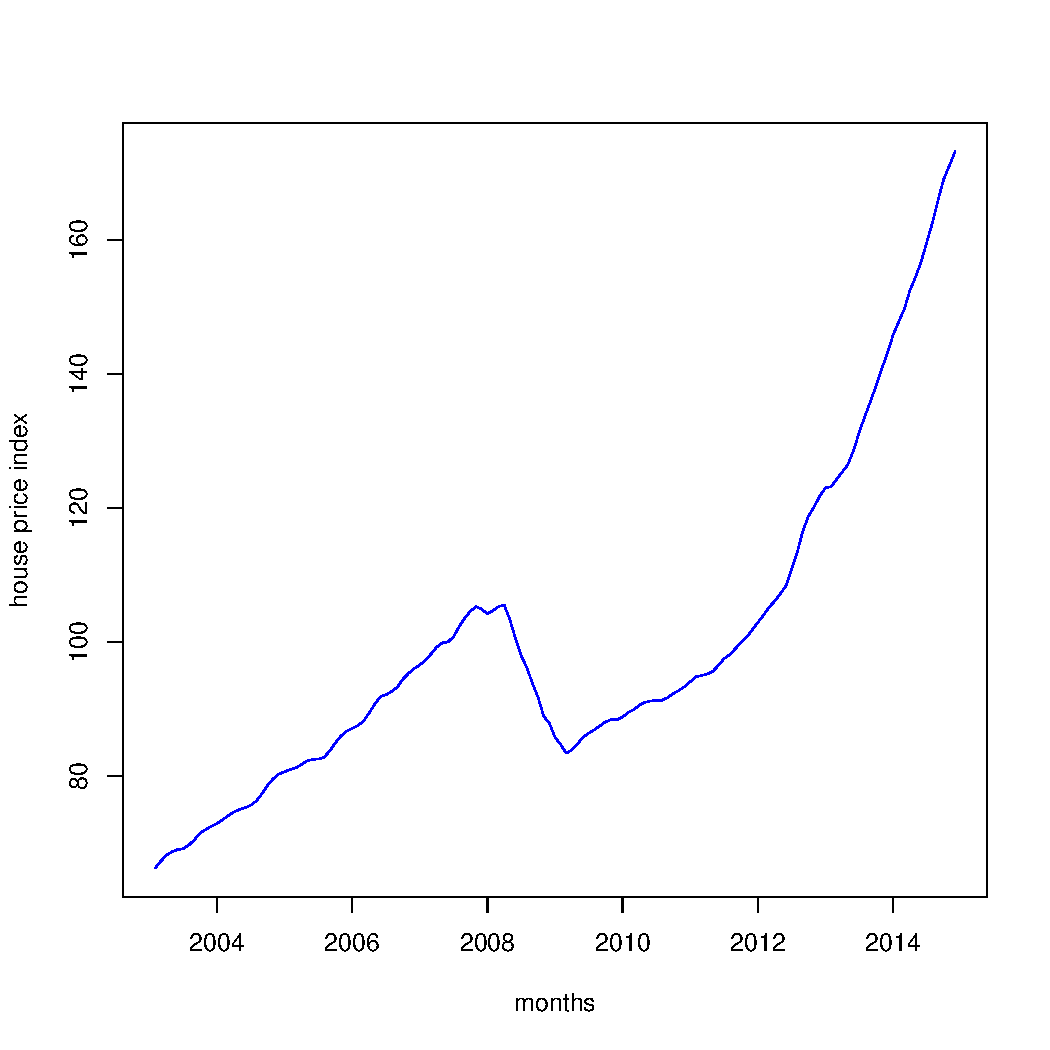
\includegraphics[scale=0.25]{figs/reidin.pdf}
		\caption{Reidin Turkish house price index}
\end{figure}

\framebreak

	\item Wage dynamics are obtained from TUIK Houshold Budget Survey (HBS) and Aktug, Kuzubas, Torul (2017) (notice the hump shape):

\begin{figure}[h]
	\centering
	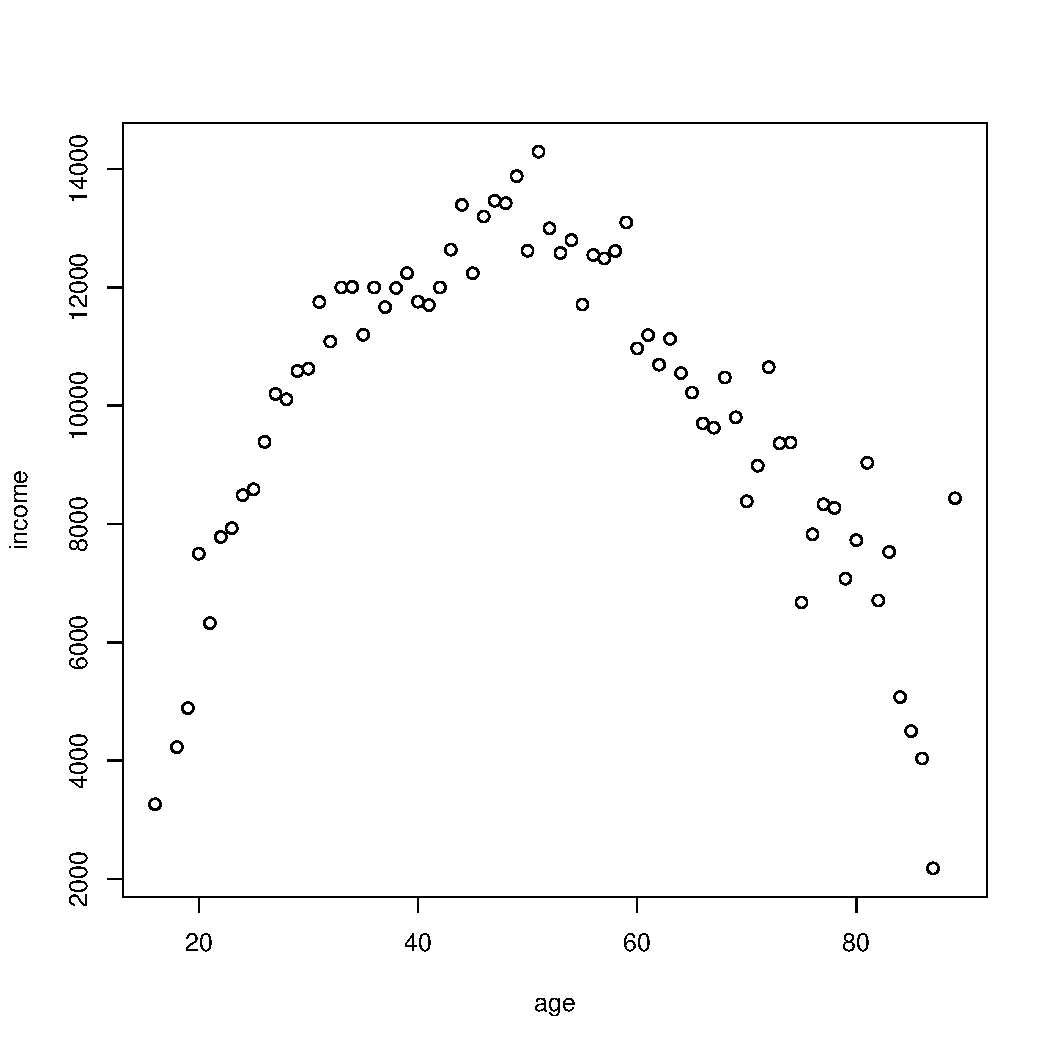
\includegraphics[scale=0.25]{figs/wage2median.pdf}
	\caption{Median Turkish salaries by age}
\end{figure}

\framebreak

	\item We start with 25 years old individual, who invests for 40 years until retirement at 65.
	\item The investments are done from $3\%$ of every wage from 25 to 64 years.
	\item In line with Torul et al. (2018), $\delta = 0.89$ and $\gamma = 1.5$ for Turkey is chosen as a default. 

\framebreak

\begin{table}
	\centering
	\caption{Benchmark Parameters}
	\begin{tabular}[c]{lll}
		\hline
		Parameter&Description&Value\\
		\hline
		$Y$&Beginning age&$25$\\
		$R$&Retirement age&$65$\\
		$T$&Lifespan (years)&$100$\\
		$\gamma$&Risk aversion&$1.5$\\
		$\beta$&Discount rate&$0.89$\\
		$r_f$&Risk-free rate&$0.03$\\
		\hline
		$\mu_s$&Expected stock returns&$0.0669$\\
		$\mu_h$&Expected housing returns&$0.0067$\\
		$\sigma_s$&Stock returns volatility&$0.3844$\\
		$\sigma_h$&Housing returns volatility&$0.0542$\\
		$\sigma_w$&Wage growth volatility&$0.036$\\
		$\rho_{hs}$&House-stock correlation&$0.24$\\
		$\rho_{hw}$&House-wage correlation&$0.37$\\
		\hline
		$p_{25}$&Survival probability at age 25&$0.978$\\
		$p_{65}$&Survival probability at age 65&$0.86$\\
		$p_{100}$&Survival probability at age 100&$0$\\	
		\hline
	\end{tabular}
\end{table}

\framebreak 
	\item The data on survival probability for all ages is obtained from TUIK database

\begin{figure}[h]
	\centering
	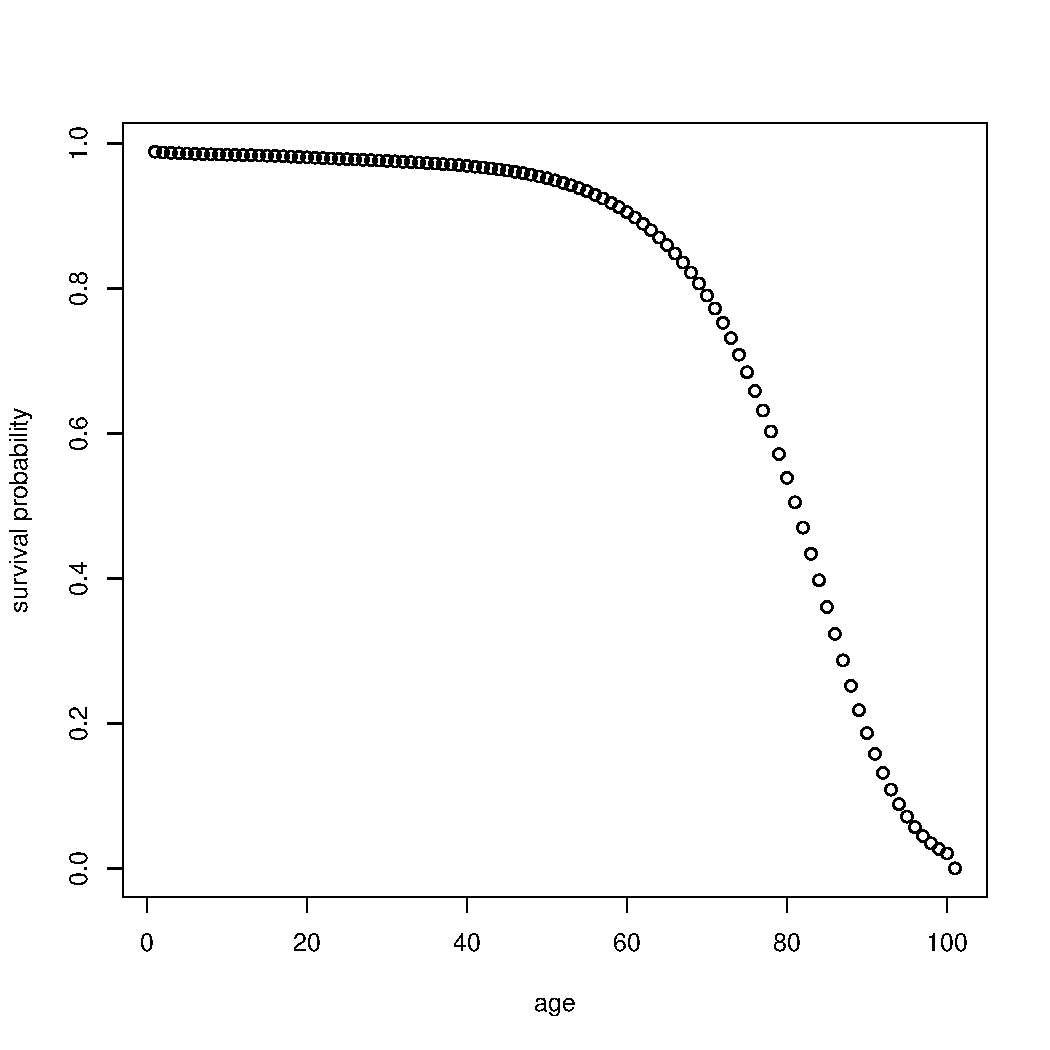
\includegraphics[scale=0.25]{figs/survival.pdf}
	\caption{Survival probabilities by age}
\end{figure}


\framebreak 

	\item We consider heterogeneity of agents as follows:
	\item Heterogeneity in education --- defined as difference in wage curve steepness

\begin{figure}[h]
	\centering
	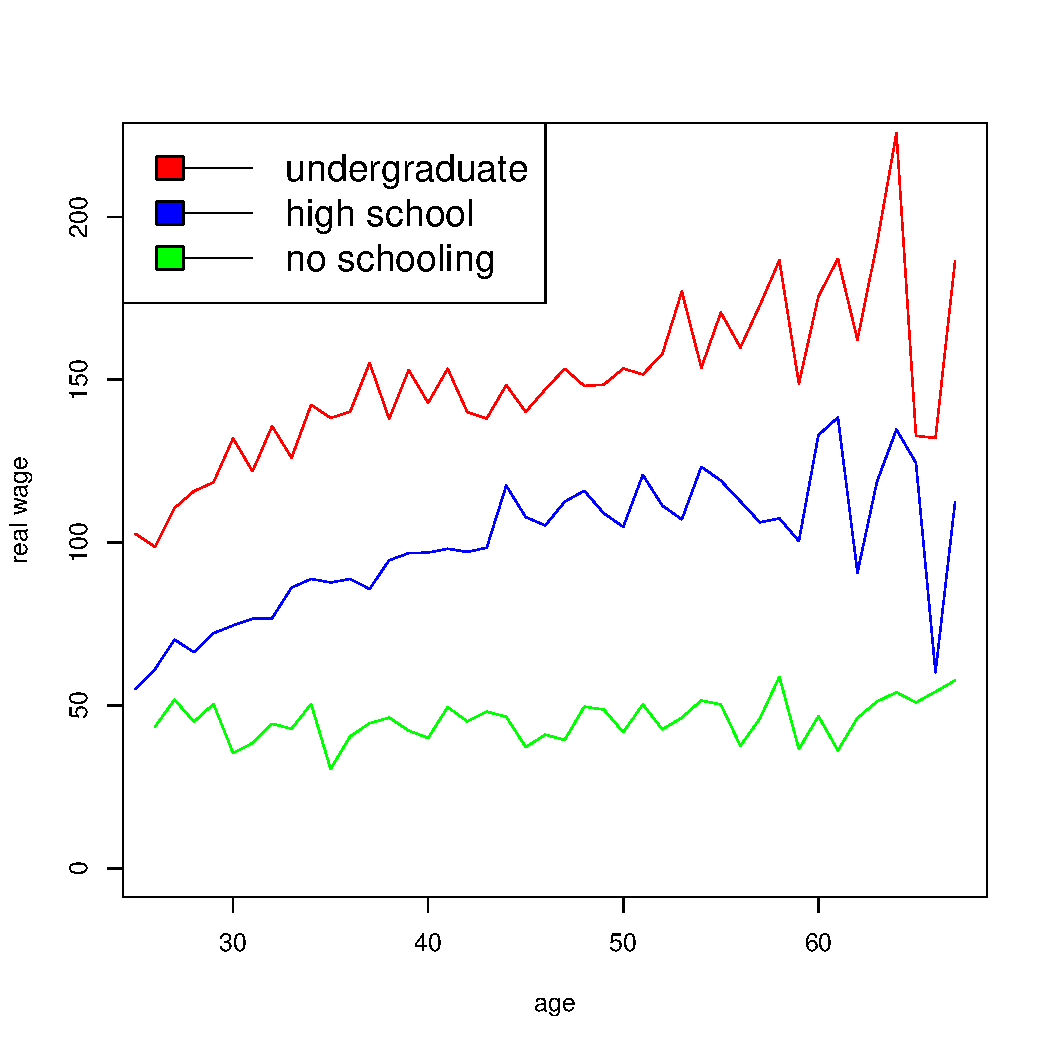
\includegraphics[scale=0.25]{figs/wage2educ.pdf}
	\caption{Lifetime wage dynamics by education level}
\end{figure}


\framebreak
	\item We use undergraduate, high school, and no schooling, to model ``steep'', ``moderate'', and ``flat'' wages.
	\item Performing regressions of wages on age, with kinks at $t=40$ and $t=55$:

\begin{equation}
	\Delta \log (wage_{it}) = \alpha_0 + \alpha_1 \cdot d_{40} + \alpha_2 \cdot d_{55}
\end{equation}

\begin{table}
	\centering
	\caption{Estimated Benchmark Wage Growth Rates $\mu_w$}
	\begin{tabular}[c]{l|ccc}
		Age&Flat&Moderate&Steep\\
		\hline
		25-40&0\%&3.8\%&2.2\%\\
		41-55&0\%&1.4\%&1.2\%\\
		56-65&0\%&0\%&1.5\%\\
	\end{tabular}
\end{table}

\framebreak

	\item Parameterized and actual wage curves

\begin{figure}[h]
		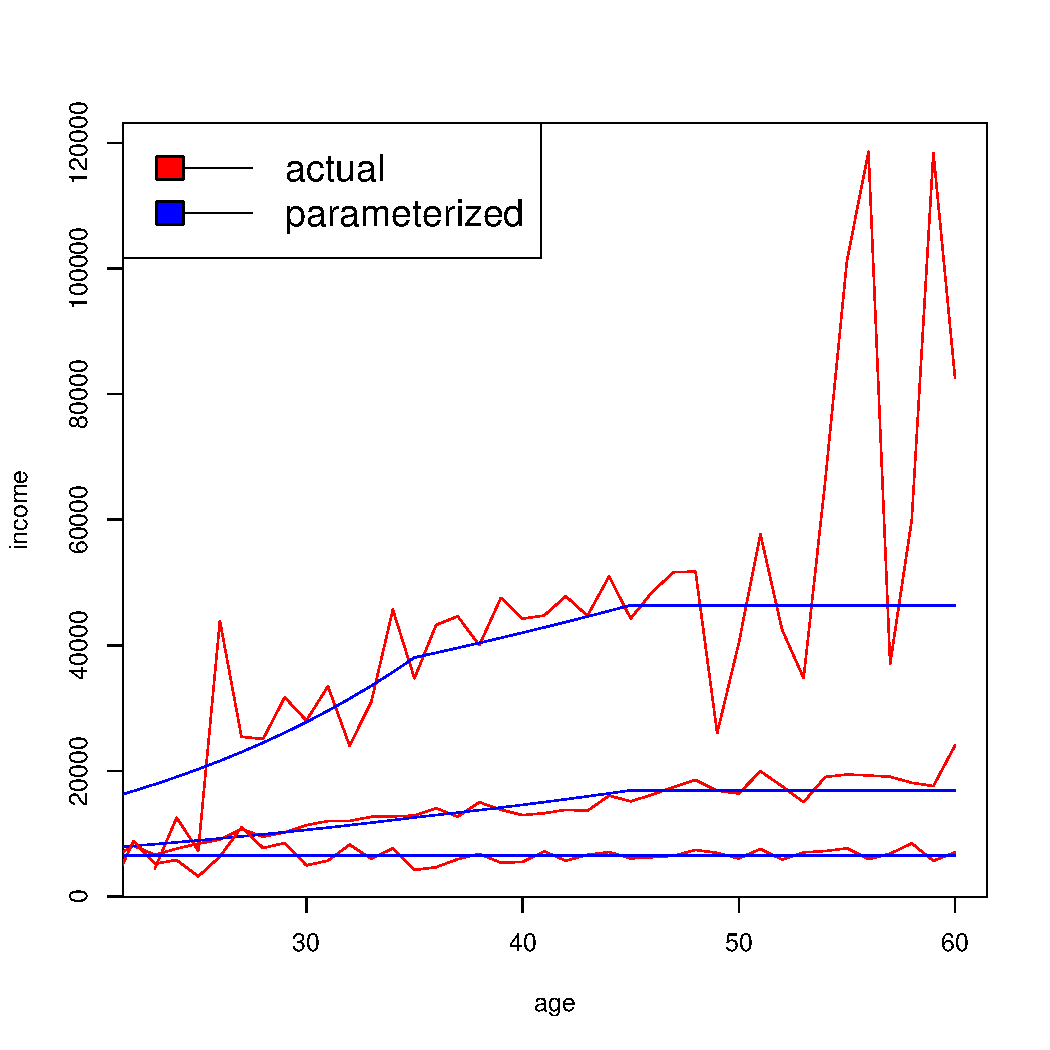
\includegraphics[scale=0.25]{figs/heterwage.pdf}
		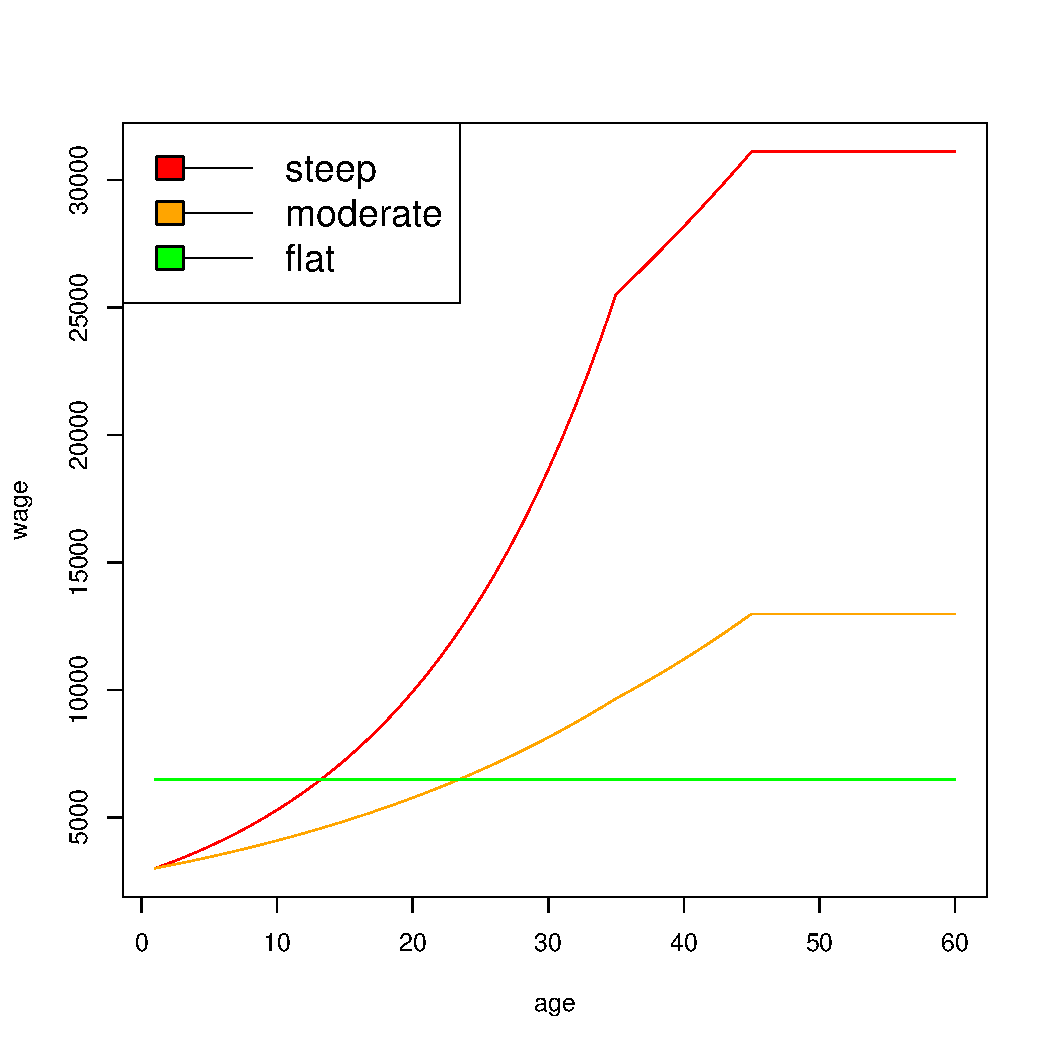
\includegraphics[scale=0.25]{figs/heterwageless.pdf}
\end{figure}

	\item Starting salary: 100 for steep wages, 50 for moderate and flat.

	\framebreak

	\item Heterogeneity in sectors of work --- it is captured by differing stock-wage correlations
	\item Zero for agricultural sector / teaching
	\item As high as $0.4$ for financial sector
	\item $0.2$ in the middle
	\item Notice movements during 2008 crisis

\begin{figure}[h]
	\centering
	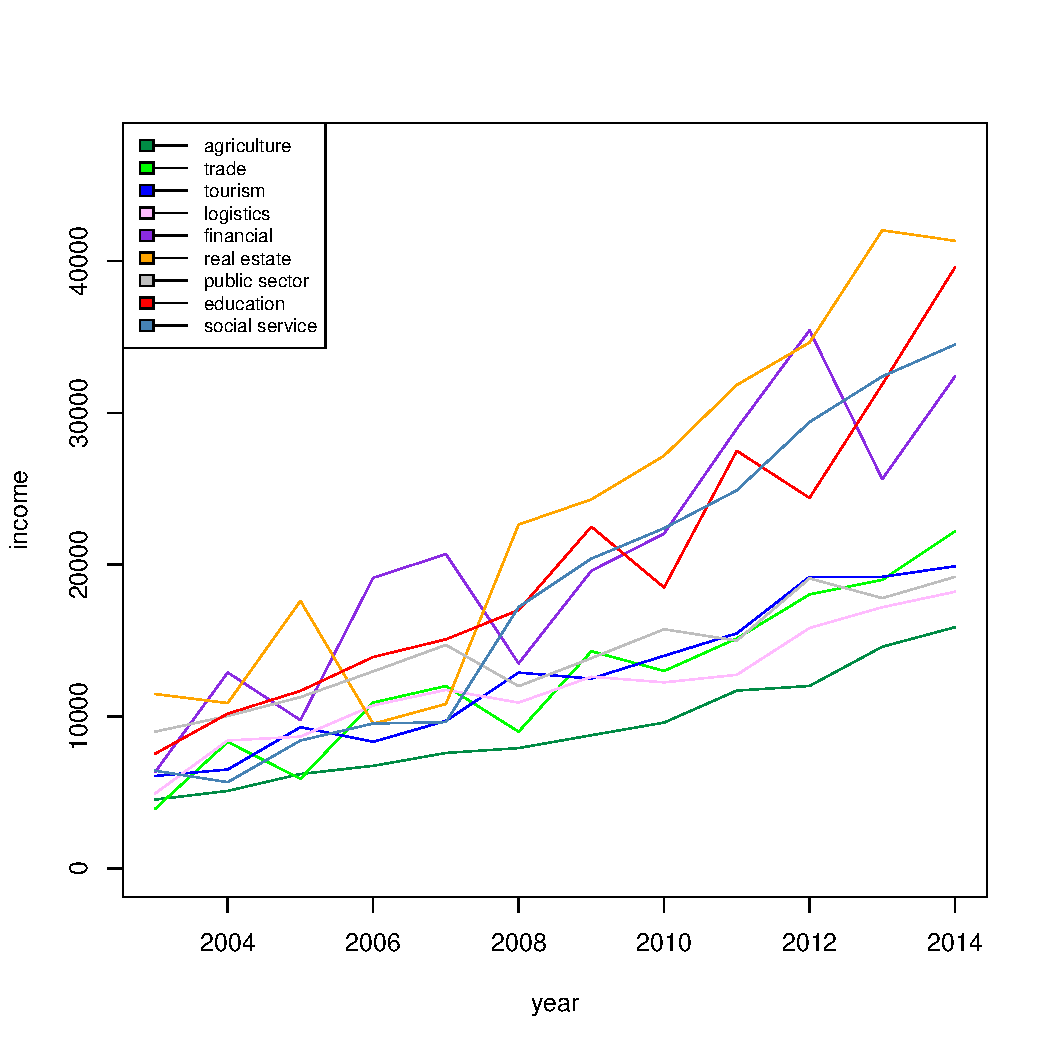
\includegraphics[scale=0.3]{figs/wage2sec.pdf}
	\caption{Historical wage dynamics by sector}
\end{figure}

\framebreak

	\item Individual heterogeneity --- it is captured by different risk aversion levels:

\begin{table}
	\centering
	\caption{Coefficients of Risk Averion}
	\begin{tabular}[c]{r|cccc}
		Values&default&low&moderate&high\\
		\hline
		$\gamma$&1.5&3&5&10\\
	\end{tabular}
\end{table}
	
\framebreak

	\item We constructed human capital and financial capital series taking the heterogeneities into consideration:
	\item $L_t/F_t$ is declining in $t$ --- optimal risky asset share is declining

\begin{figure}[h]
		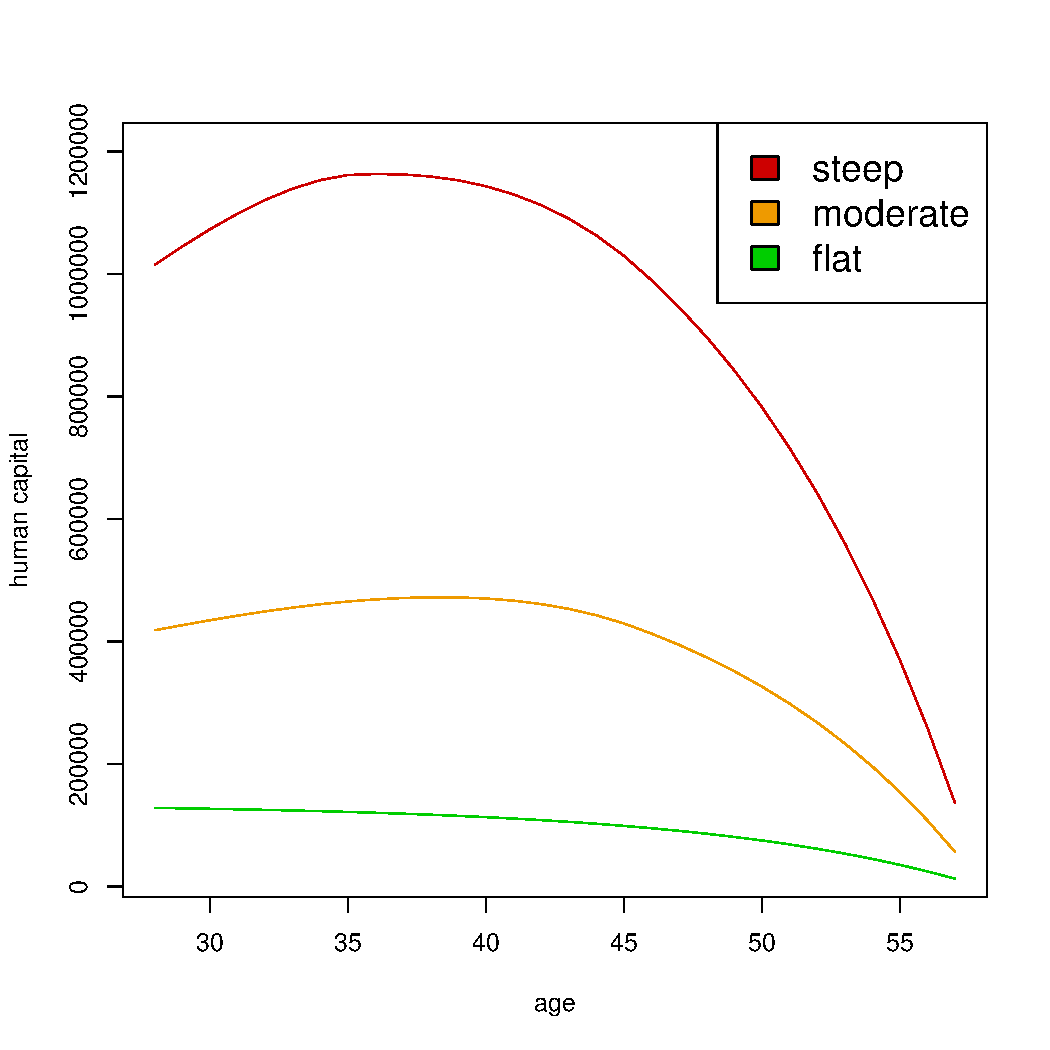
\includegraphics[scale=0.25]{figs/humancapital.pdf}
		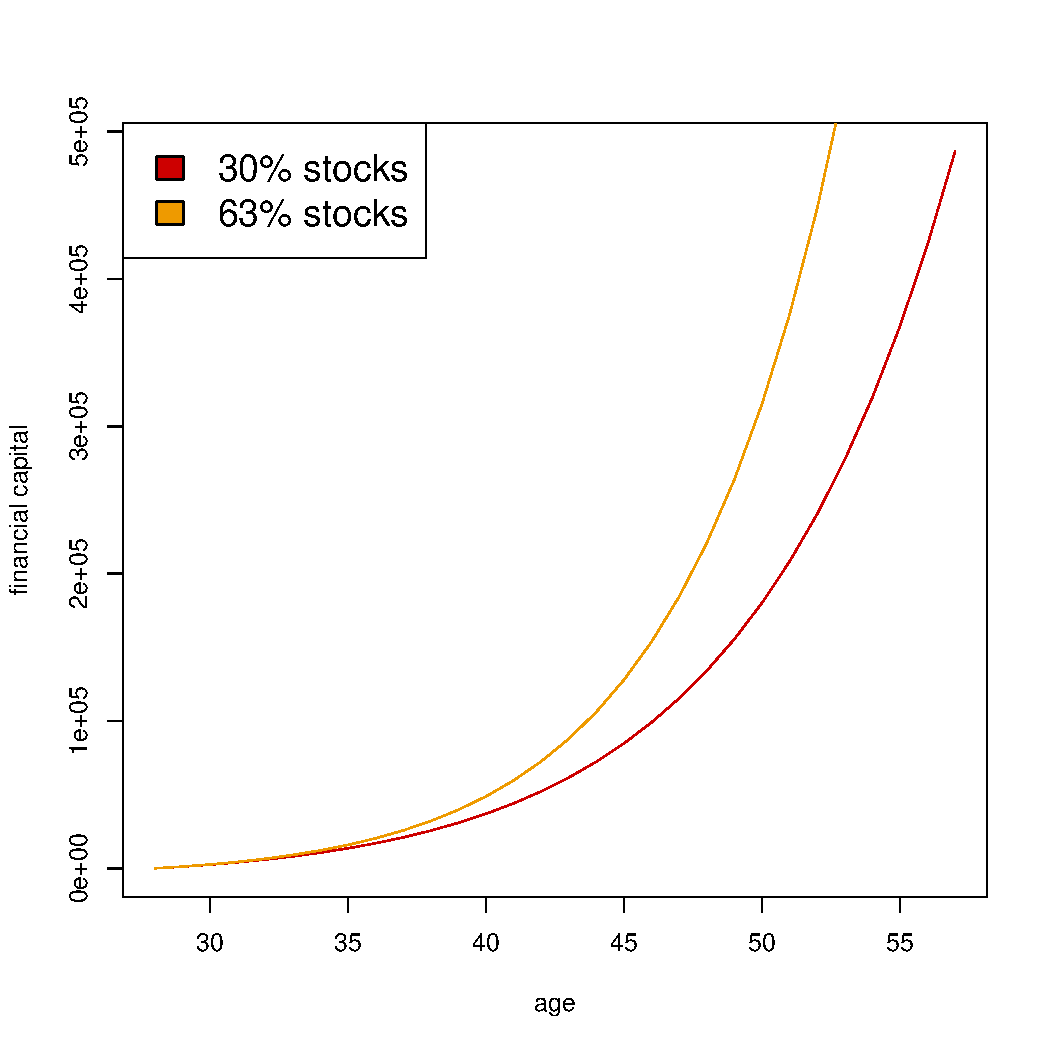
\includegraphics[scale=0.25]{figs/fincapital.pdf}
\end{figure}

\begin{figure}[h!]
	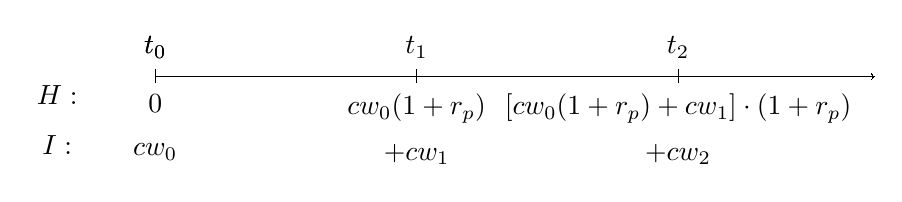
\begin{tikzpicture}[scale=0.83]
		\draw [->, line width=0.mm] (0,0) -- (11,0);
		\foreach \x in {0,4,8}
			\draw (\x cm,3pt) -- (\x cm, -3pt);
		\draw (0,0) node[below=21pt] {$ cw_0 $} node[above=3pt] {$ t_0 $};
    	\draw (4,0) node[below=21pt] {$ +cw_1 $} node[above=3pt] {$ t_1 $};
    	\draw (8,0) node[below=21pt] {$ +cw_2 $} node[above=3pt] {$ t_2 $};
		\draw (0,0) node[below=3pt] {$ 0 $} node[above=3pt] {$ t_0 $};
    	\draw (4,0) node[below=3pt] {$ cw_0(1+r_p) $};
    	\draw (8,0) node[below=3pt] {$ \left[cw_0(1+r_p) + cw_1 \right] \cdot (1+r_p) $};
	    \draw (-1.5,0) node[below=18pt] {$I:$};
    	\draw (-1.5,0) node[below=0pt] {$H:$};
	\end{tikzpicture}
	\caption{Law of motion of financial capital. Every period, a certain percentage $c$ of the wage $w_t$ is invested in a retirement portfolio, while the previously invested amount accrues interest at portfolio rate of return $r_p$.}
	\label{fig:invdiag}
\end{figure}

  \end{itemize}
\end{frame}

\section{All Strategies}

\begin{frame}[allowframebreaks]{Strategies}
  \begin{itemize}
	\item First, we list default and derived investment strategies
	\item Then we calculate the capital movements using these strategies
	\item We obtain total wealth before retirement and annuitize it
	\item We convert annuities into consumption levels considering inflation
	\item We plug consumption levels into expected utilities
	\item We compare resulting utilities and conclude

\framebreak

	\item Homogeneous strategies

\begin{figure}[h]
	\centering
	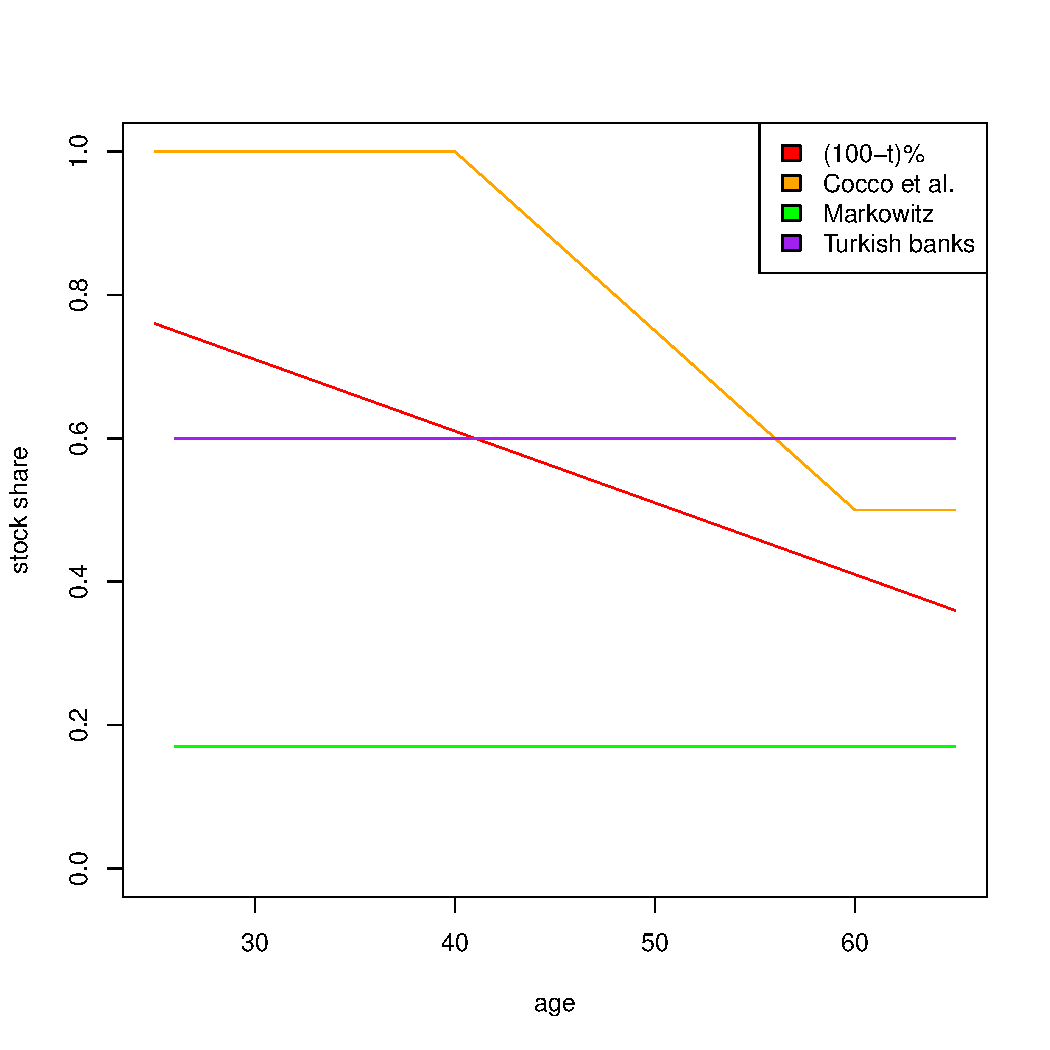
\includegraphics[scale=0.25]{figs/defaults.pdf}
	\caption{Default portfolio allocations of stock investments}
\end{figure}
		

\framebreak


	\item Several individualized solutions ($\gamma=1.5,3,5,10$):

\begin{figure}
		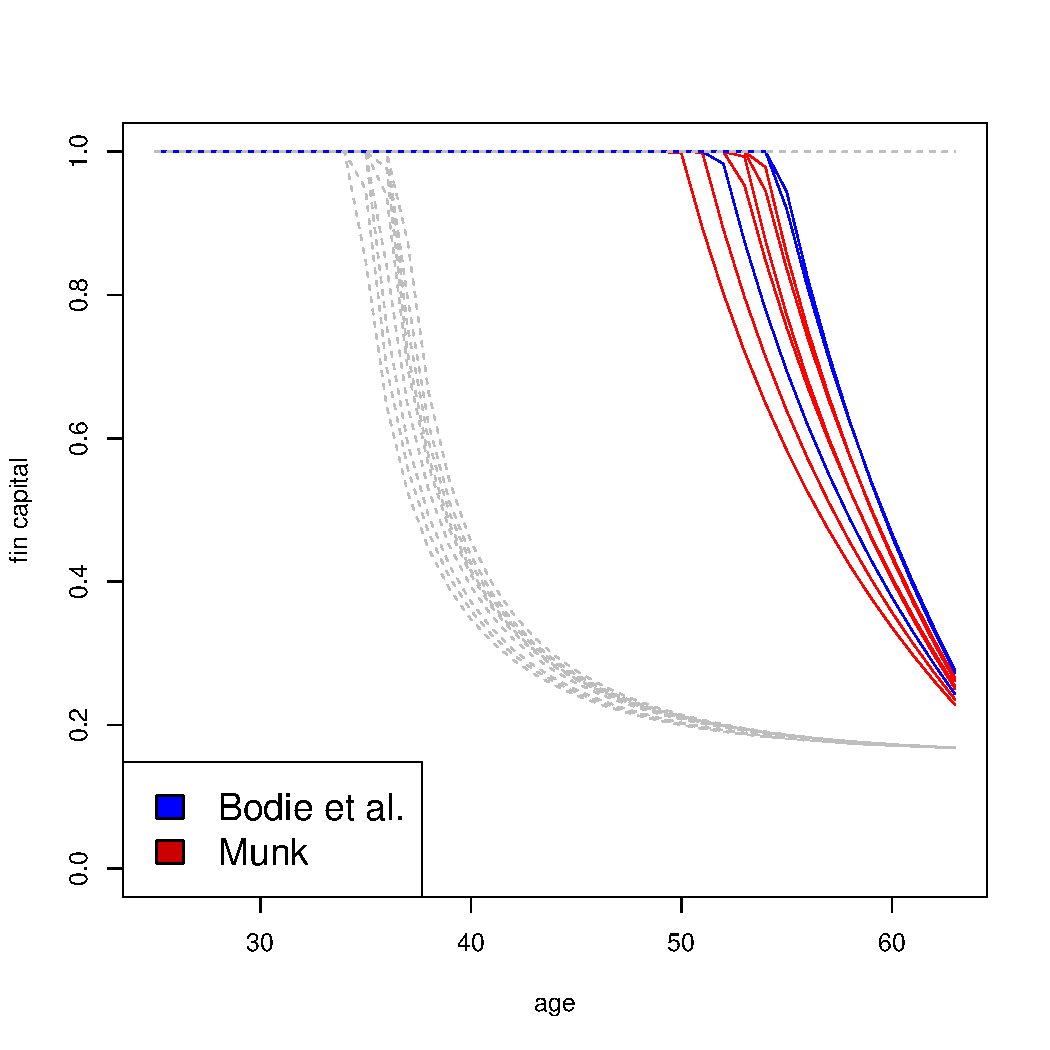
\includegraphics[scale=0.25]{figs/individuals15.pdf}
		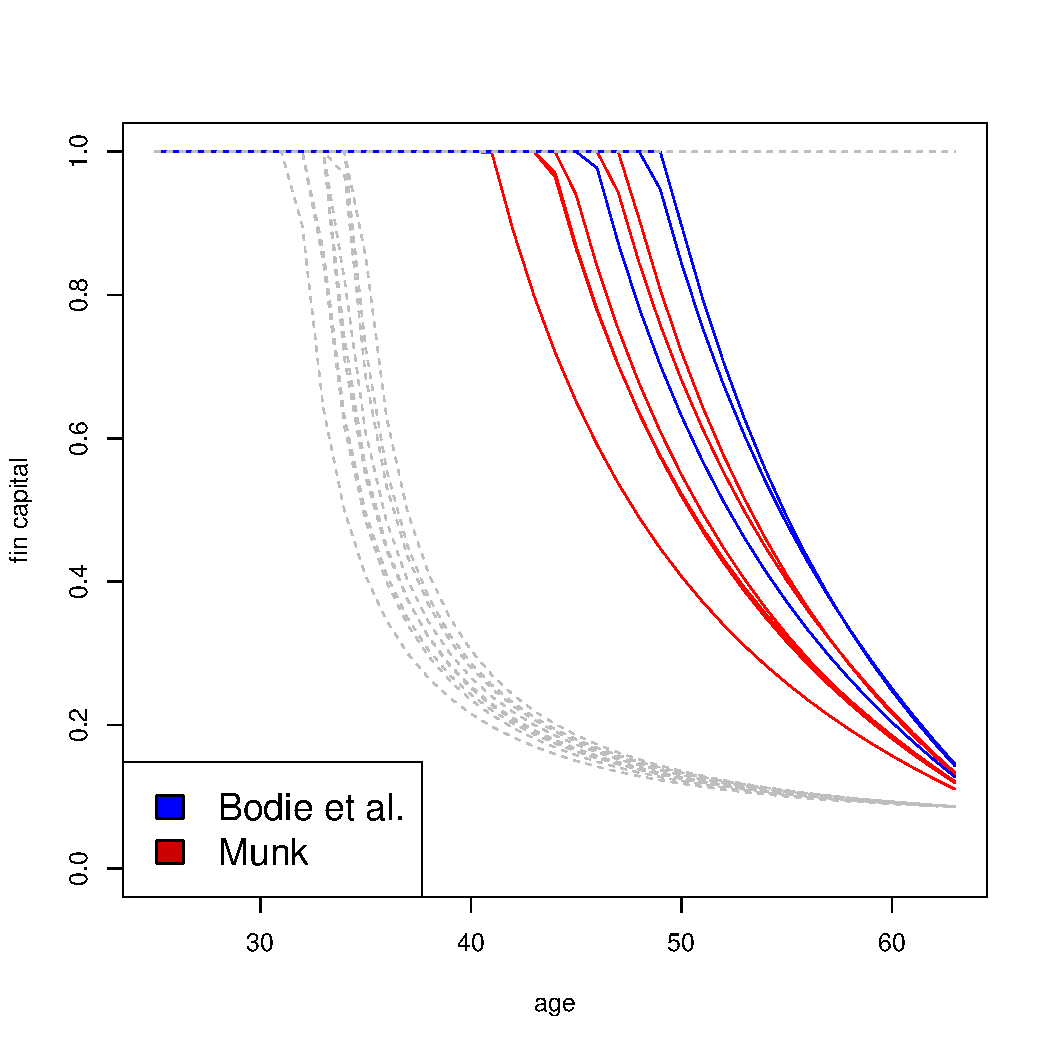
\includegraphics[scale=0.25]{figs/individuals3.pdf}
		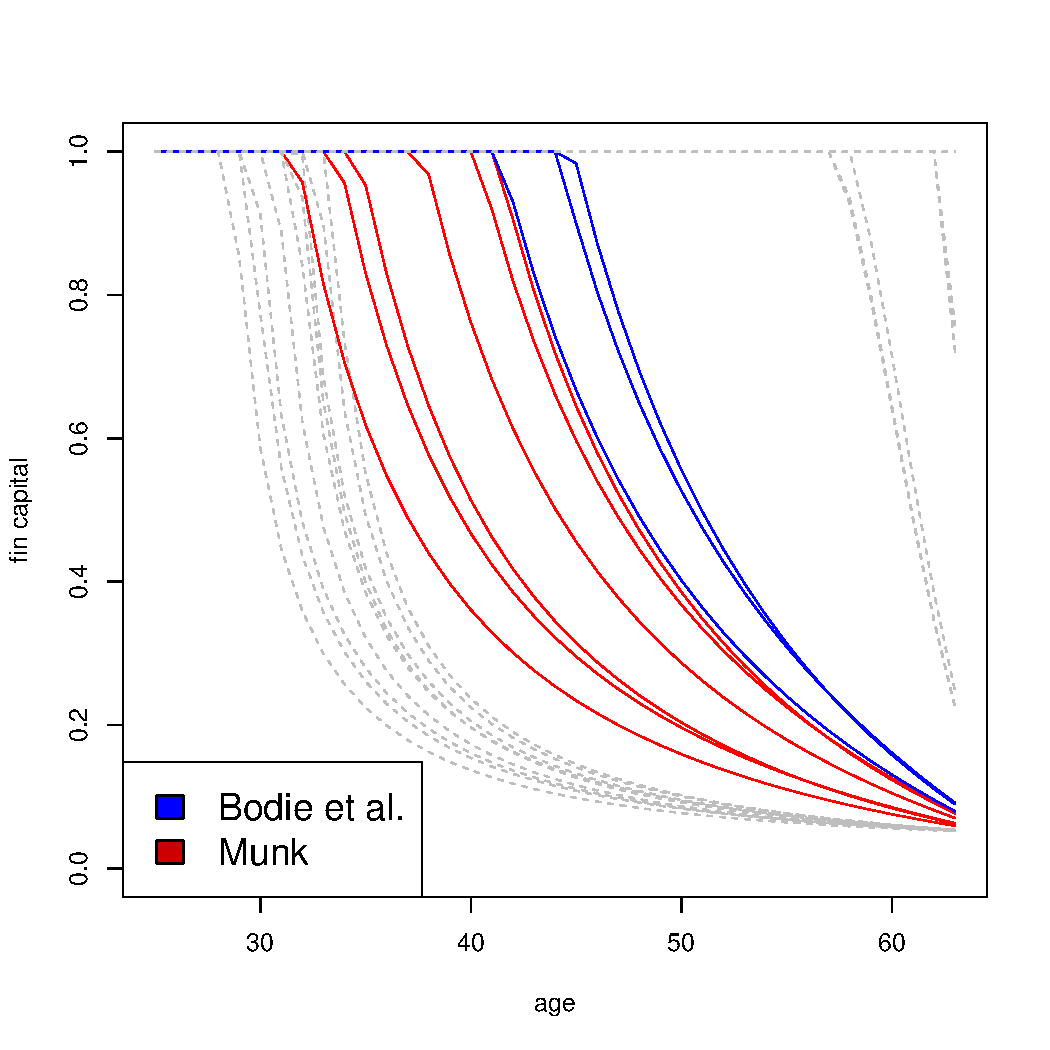
\includegraphics[scale=0.25]{figs/individuals5.pdf}
		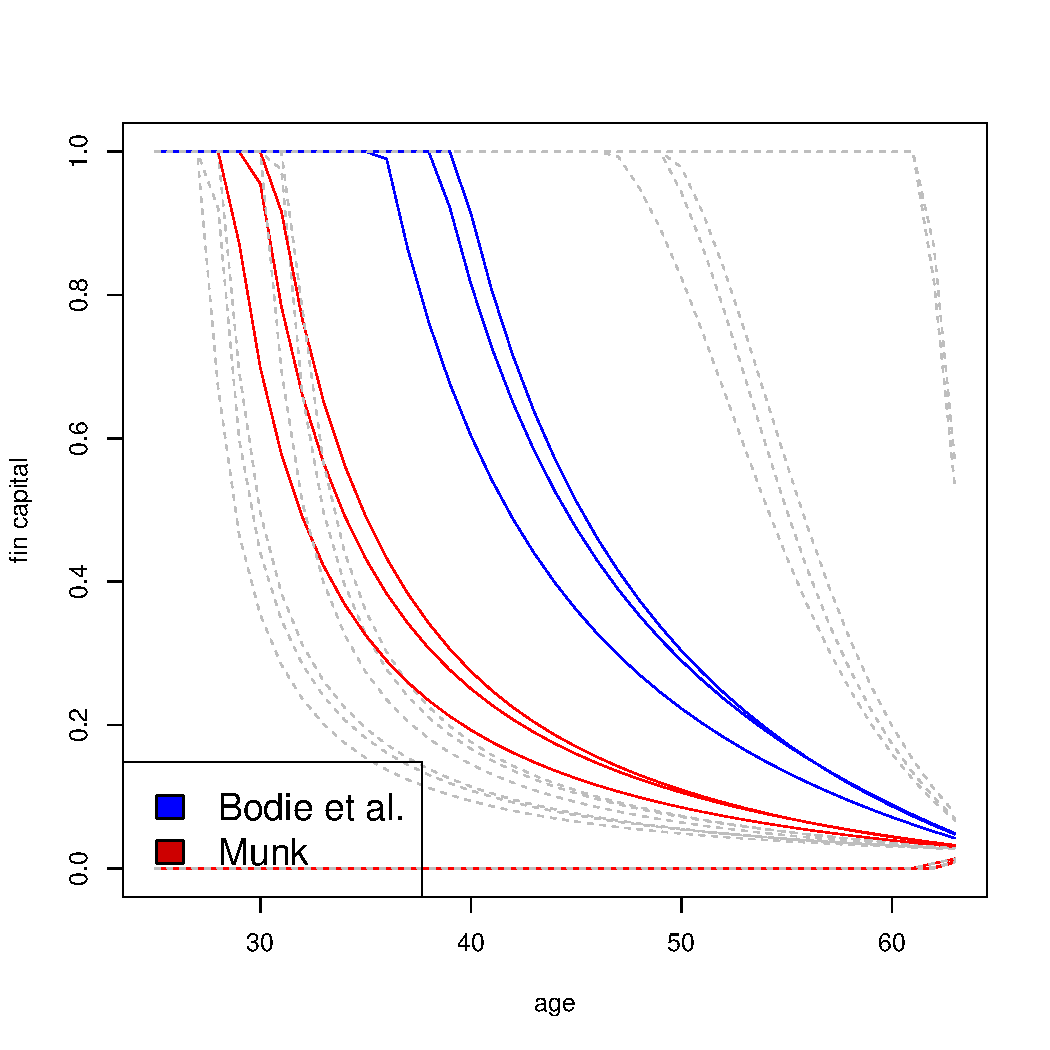
\includegraphics[scale=0.25]{figs/individuals10.pdf}
\end{figure}

\framebreak

	\item Note that for small stock-wage correlations, Munk's solution without housing is equivalent to Merton's solution
	\item Note that for smaller risk aversion, households invest more aggressively
	\item Note that flat wagers are less aggressive than steeper wagers
	\item Munk's solution with housing are presented below.
	\item Left graph is optimal stock share and right graph is optimal housing share
	\item Graphs are done for $\gamma=1.5,3,5,10$
\framebreak

\begin{figure}[H]
		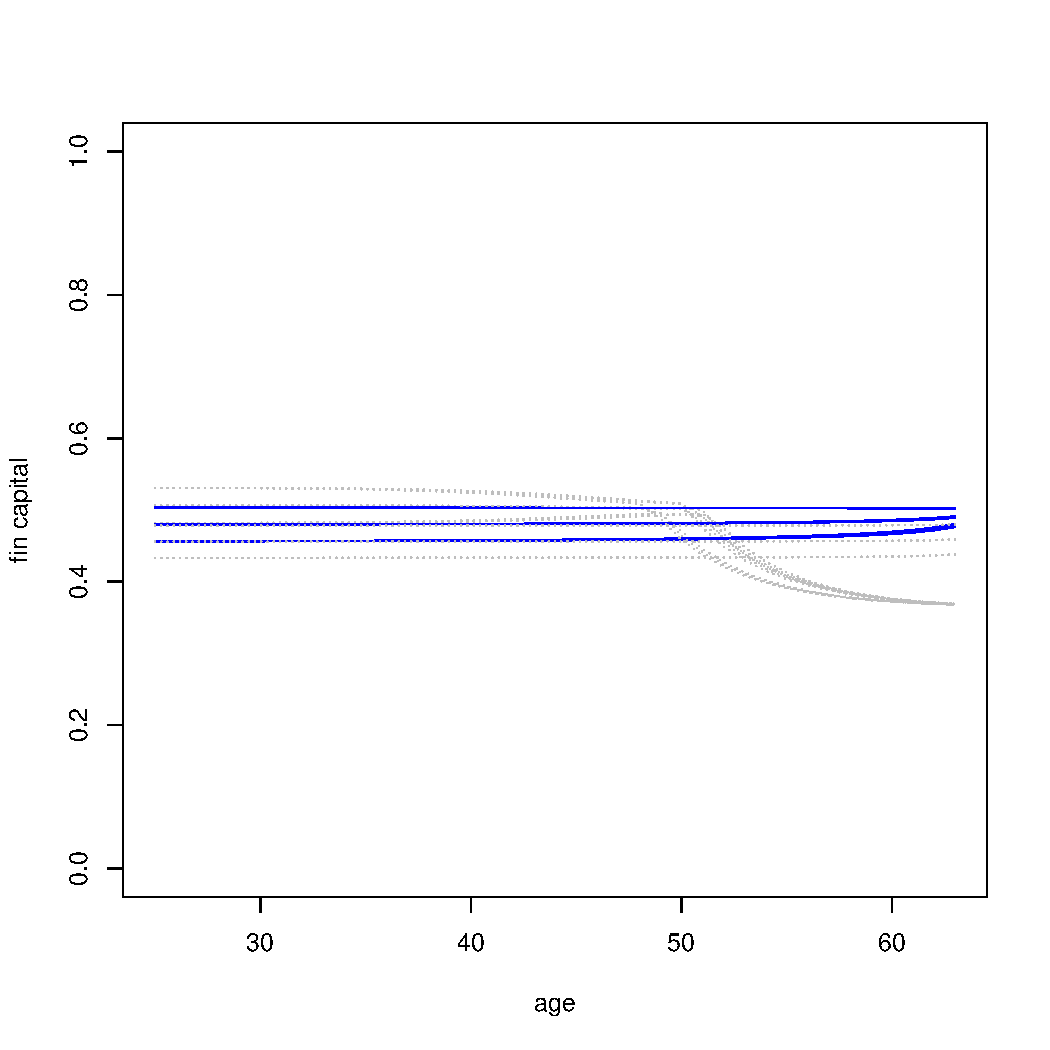
\includegraphics[scale=0.25]{figs/smunkhouse15.pdf}
		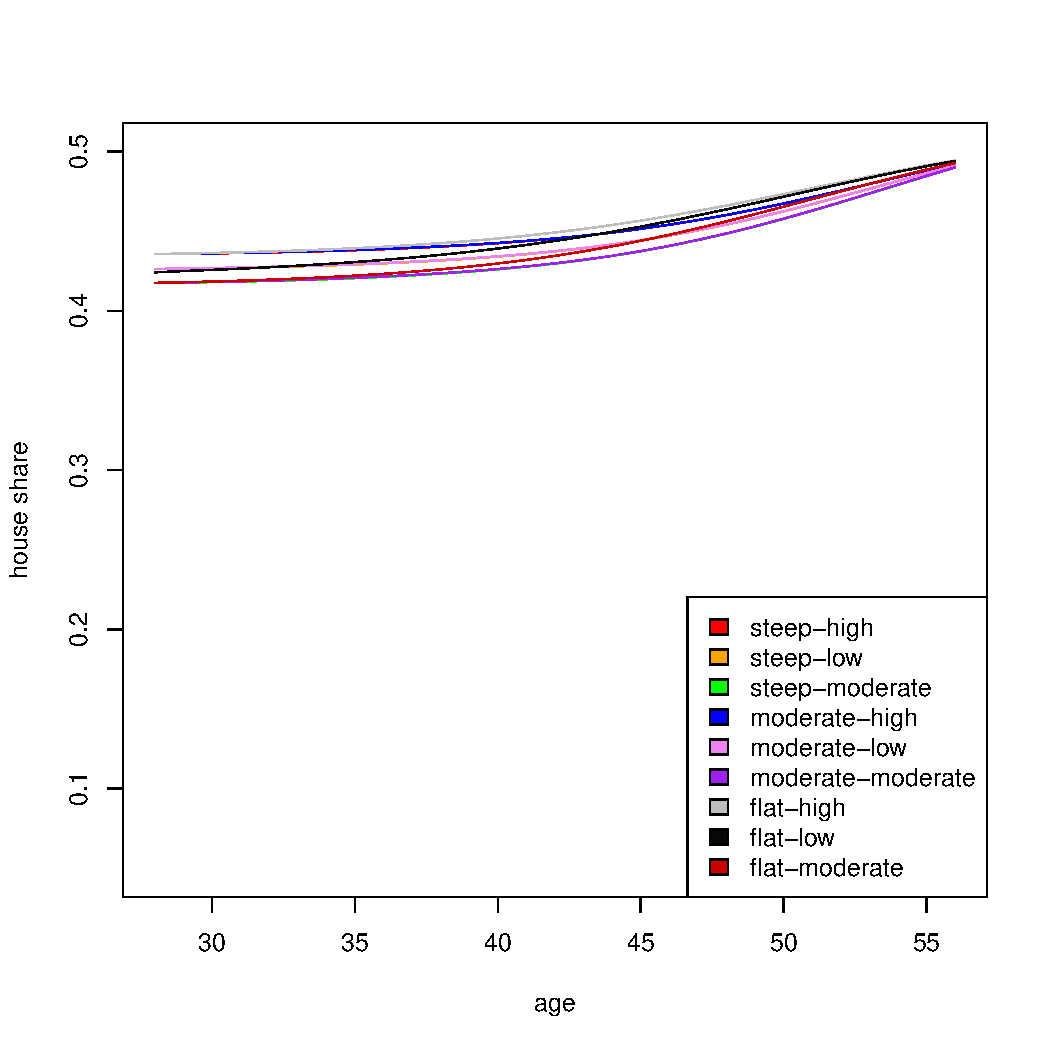
\includegraphics[scale=0.25]{figs/hmunkhouse15.pdf}
		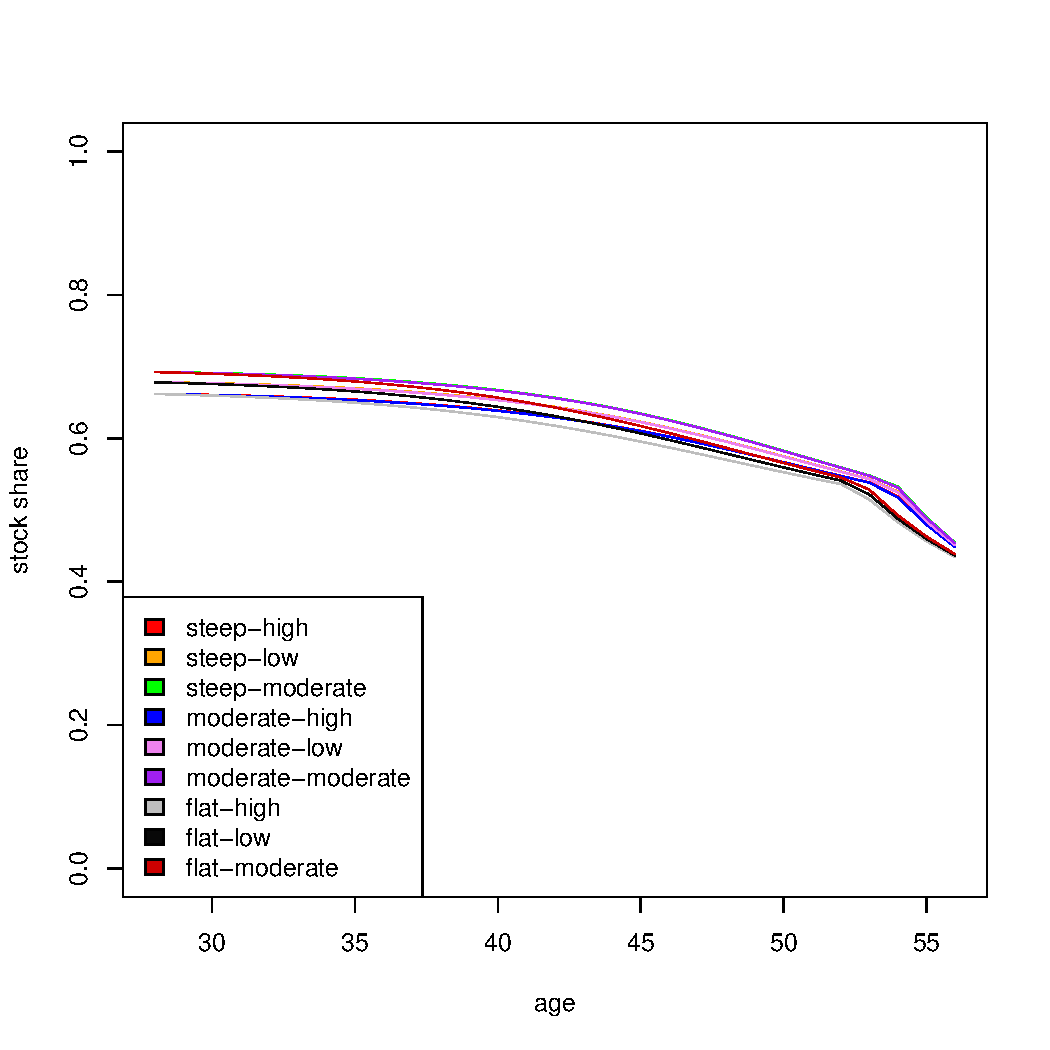
\includegraphics[scale=0.25]{figs/smunkhouse3.pdf}
		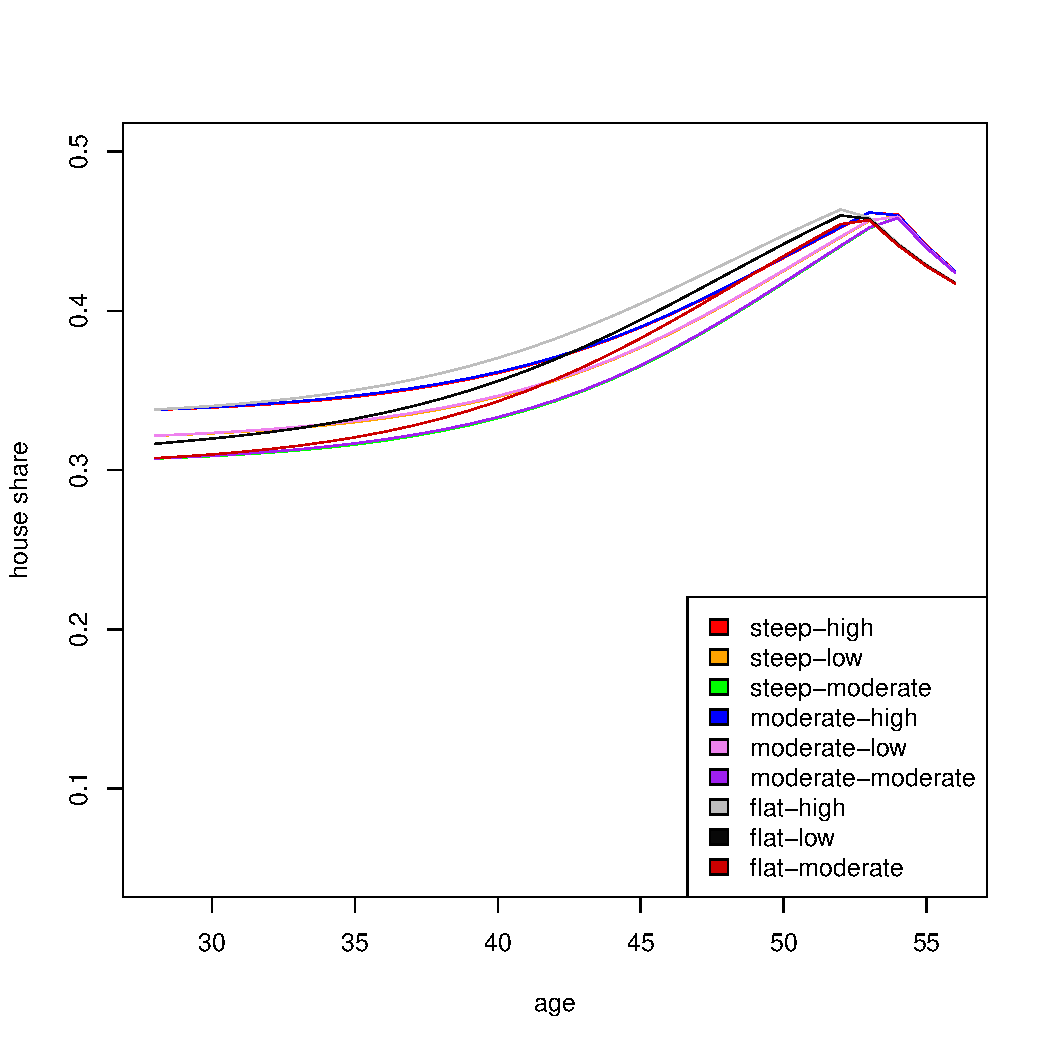
\includegraphics[scale=0.25]{figs/hmunkhouse3.pdf}
		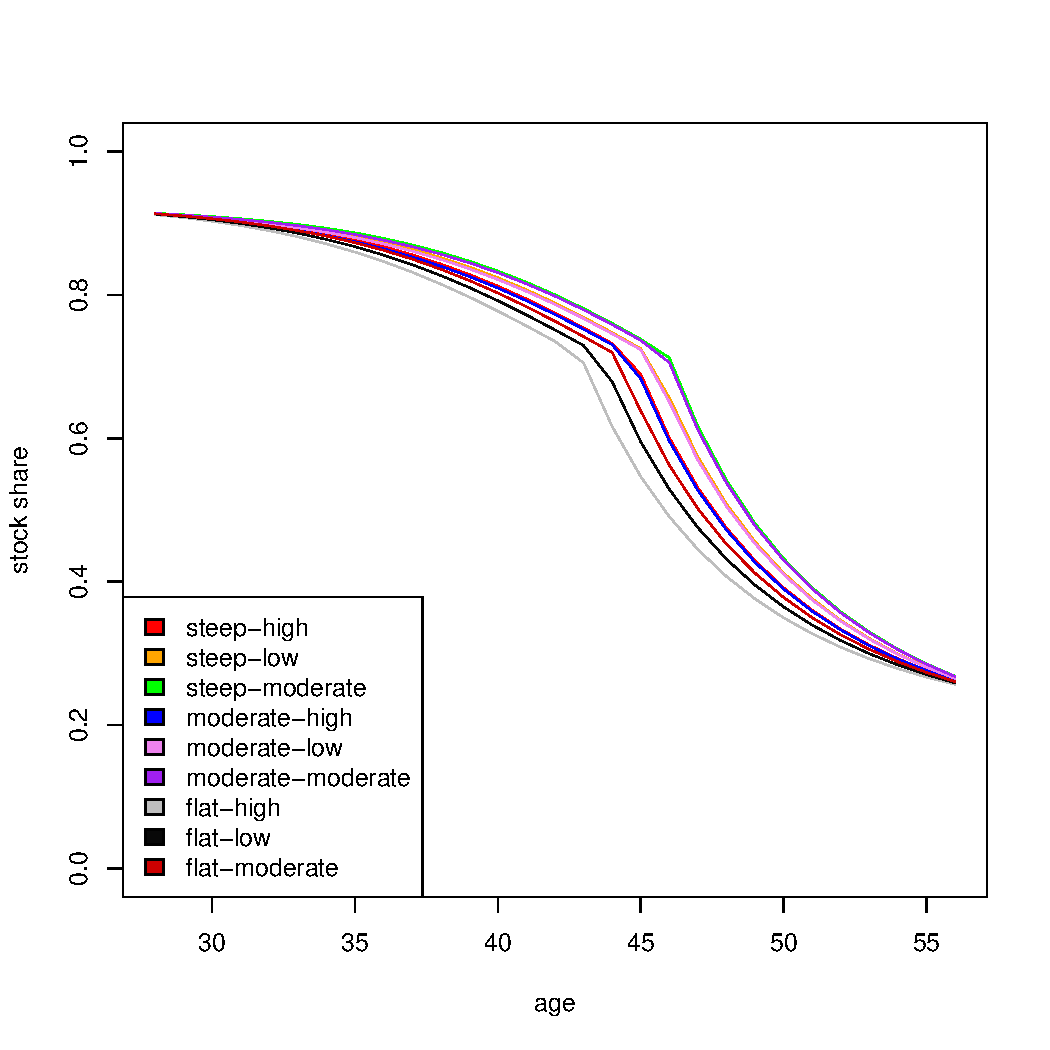
\includegraphics[scale=0.25]{figs/smunkhouse5.pdf}
		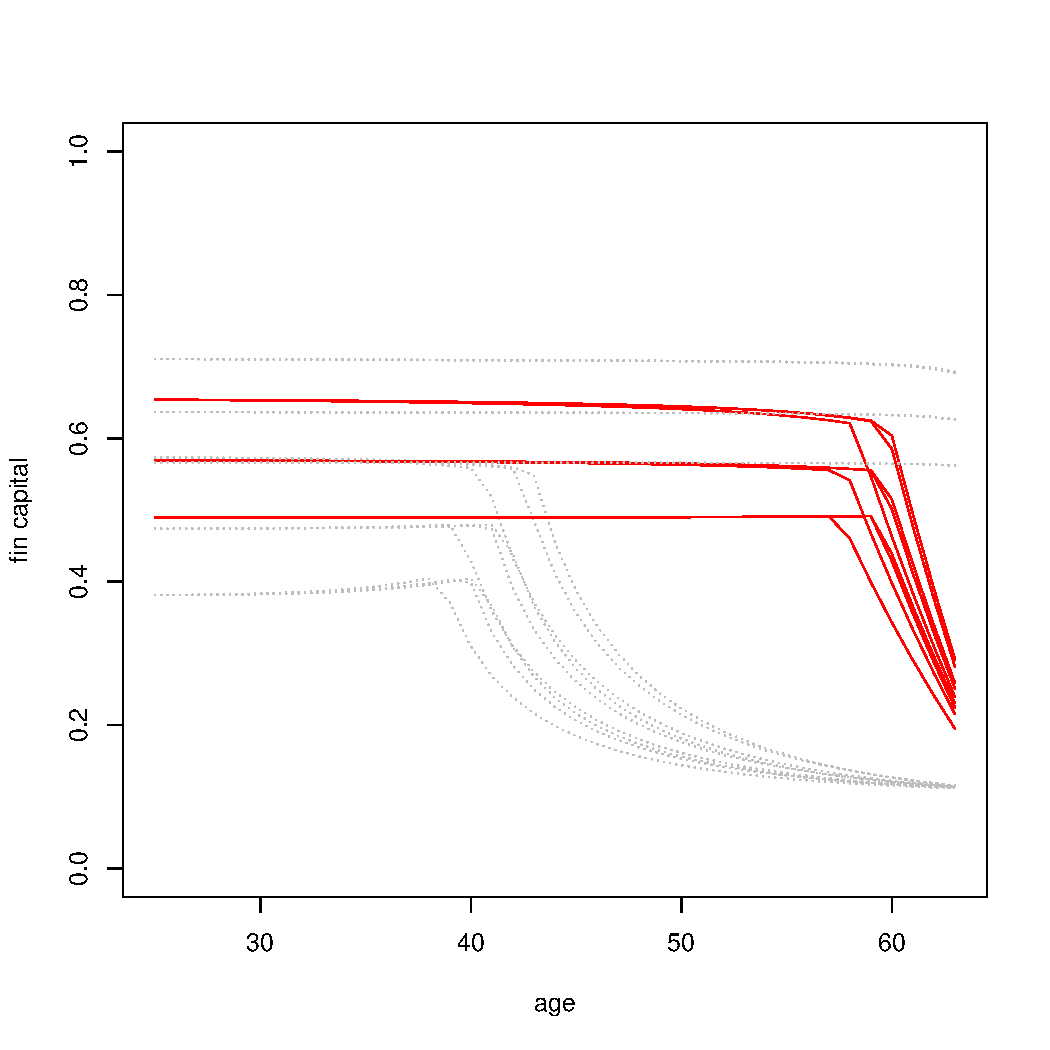
\includegraphics[scale=0.25]{figs/hmunkhouse5.pdf}
		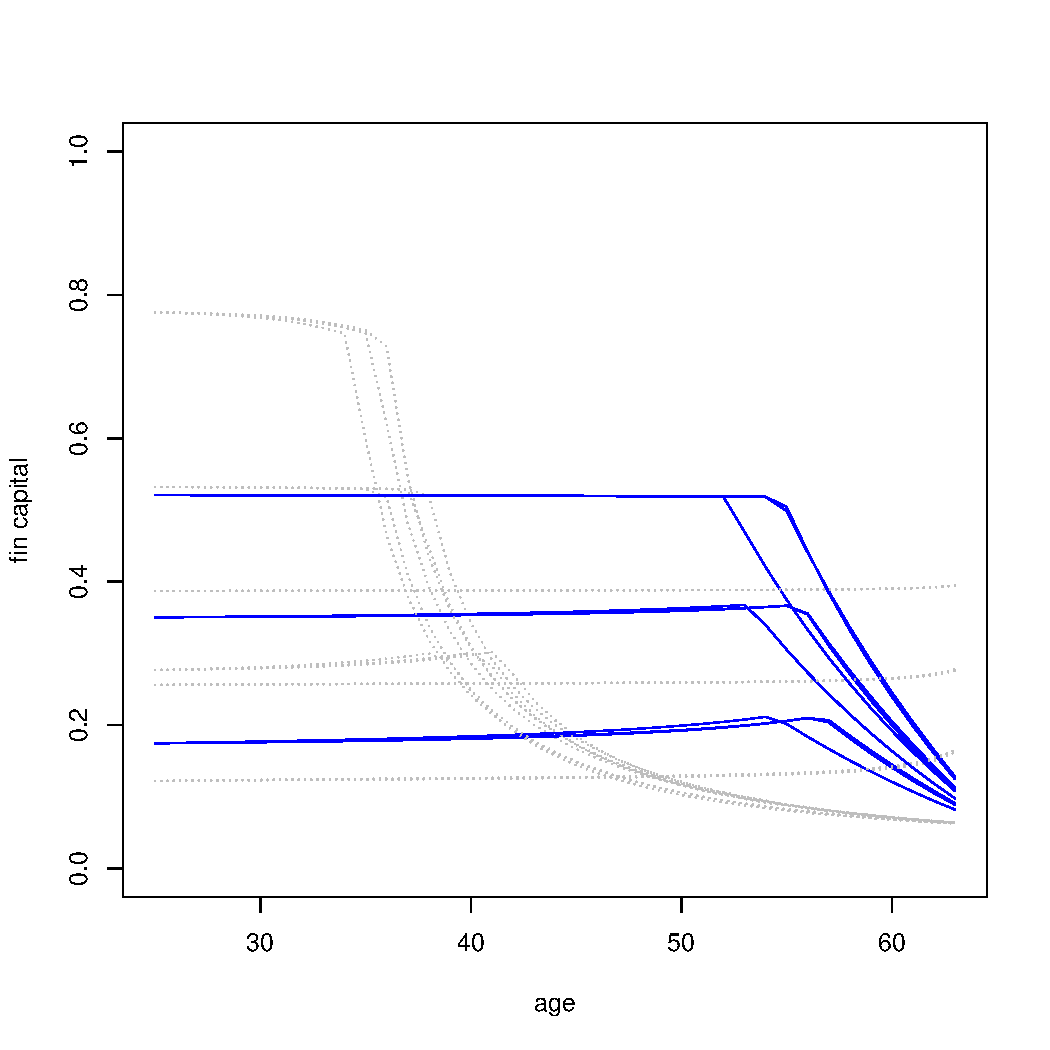
\includegraphics[scale=0.25]{figs/smunkhouse10.pdf}
		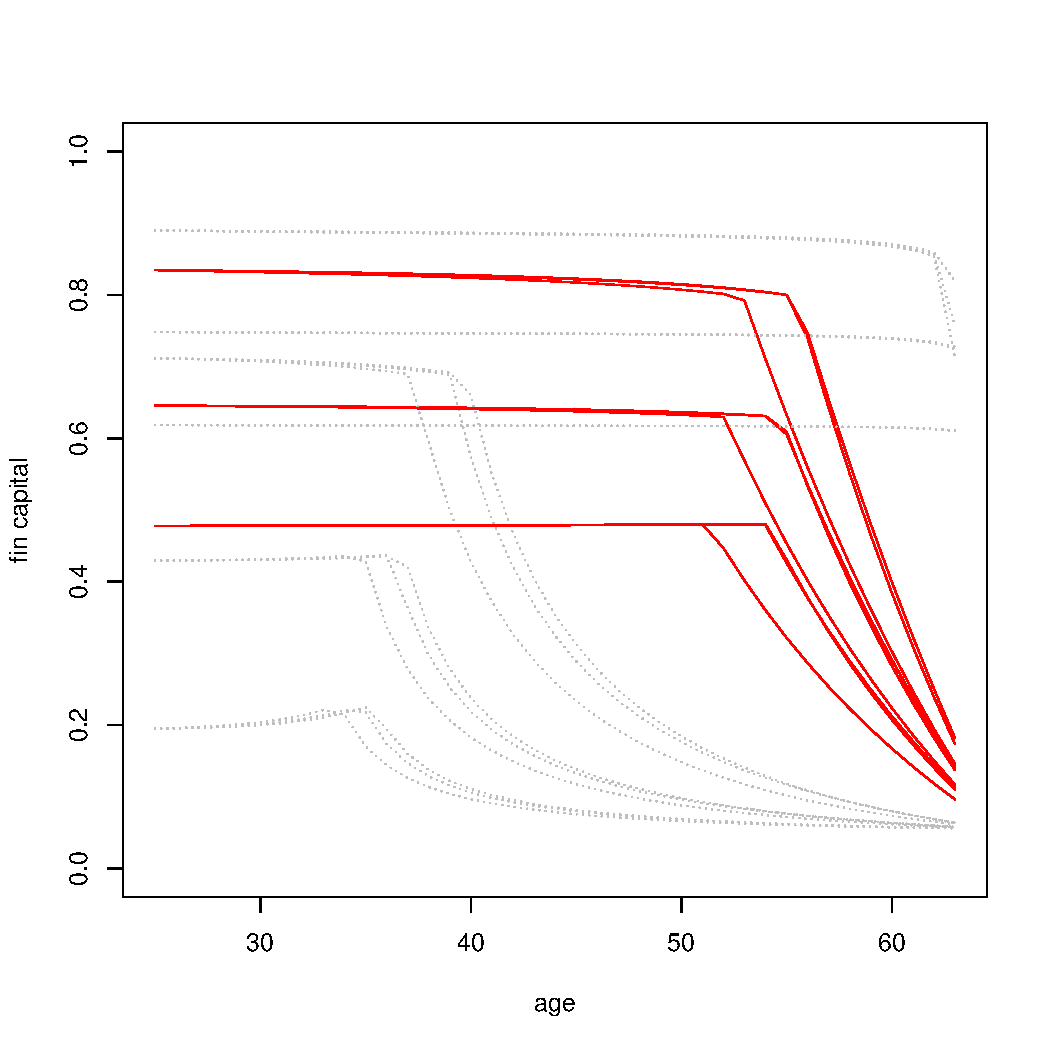
\includegraphics[scale=0.25]{figs/hmunkhouse10.pdf}
\end{figure}


\framebreak

	\item In line with Munk, the stock-house allocation is done as follows:
		\begin{itemize}
			\item If optimal stock and housing allocations sum up to a number greater than $1$, then we allocate our wealth proportionately between the two
			\item If optimal stock and housing allocations sum up to a number less than $1$, then we allocate those very shares and invest the rest into risk-free bonds 
		\end{itemize}

	\item Note that as risk aversion coefficeint increases, the kink happens earlier
	\item Note that the steeper the wage curve is, the more aggressive the individual is
	\item Note that stock-wage correlation does not influence steep and flat wagers much
\end{itemize}
\end{frame}

\begin{frame}[allowframebreaks]{Results}
  \begin{itemize}
	\begin{figure}[H]
		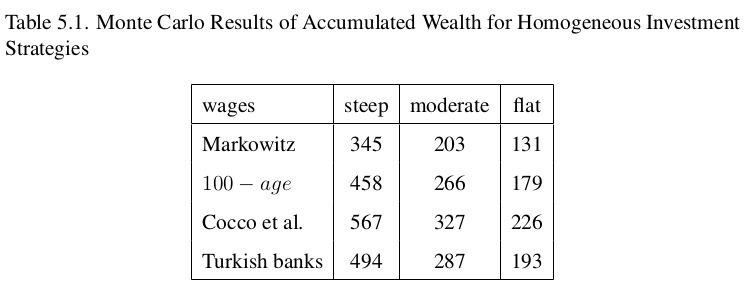
\includegraphics[scale=0.4]{figs/montecarlo_hom.png}
		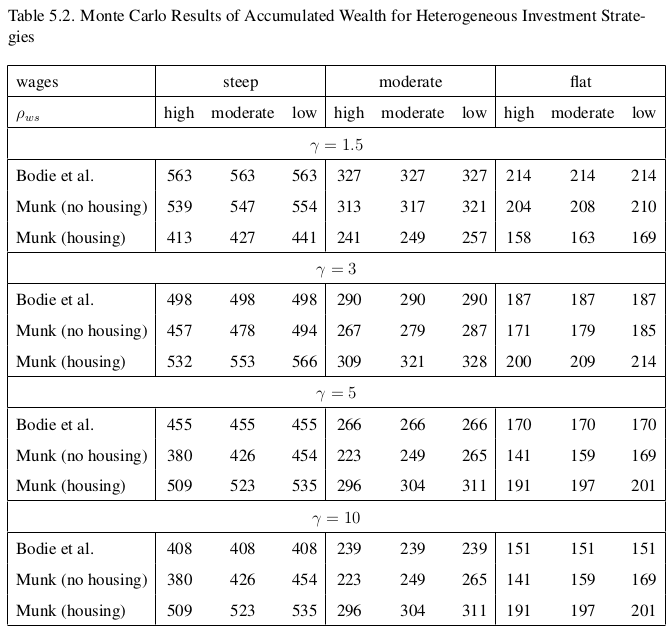
\includegraphics[scale=0.3]{figs/montecarlo_het.png}
		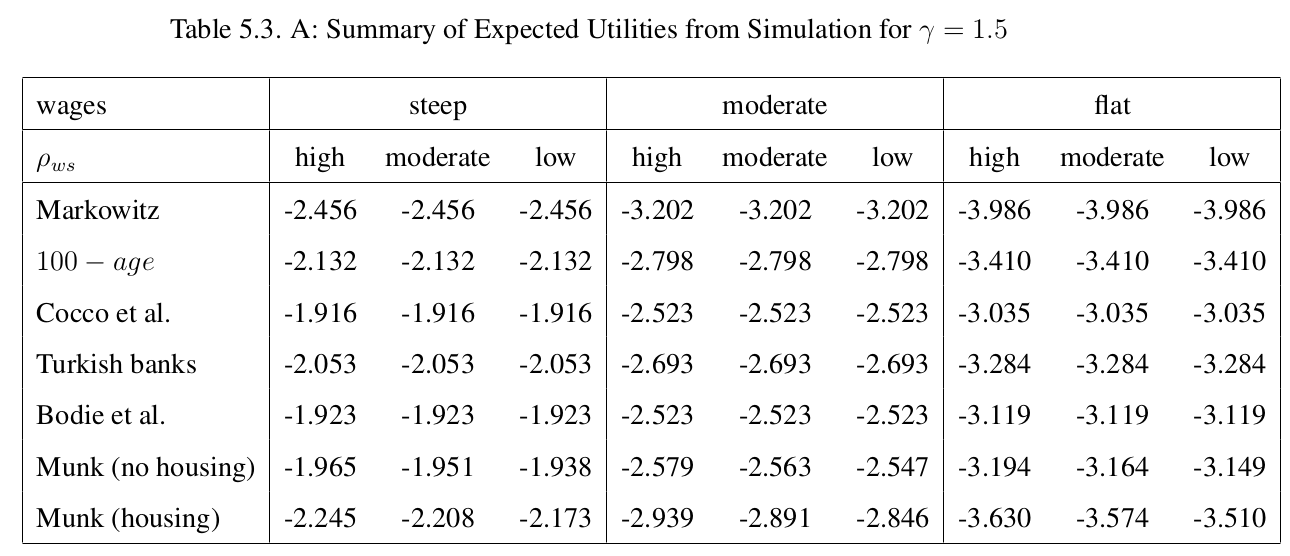
\includegraphics[scale=0.2]{figs/util15.png}
		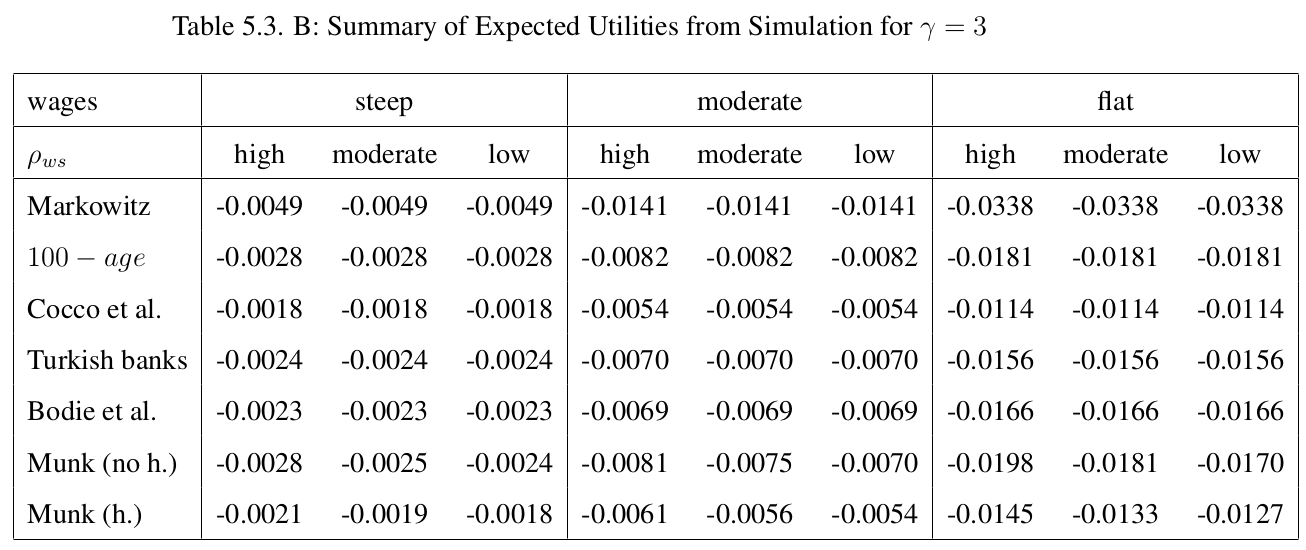
\includegraphics[scale=0.2]{figs/util3.png}
		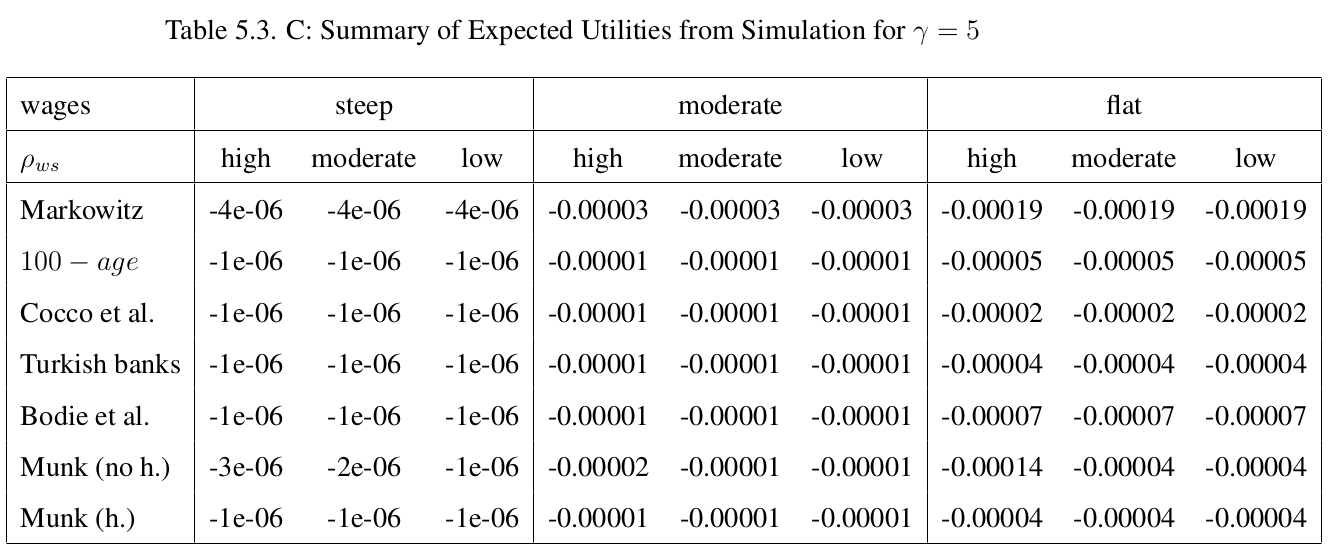
\includegraphics[scale=0.2]{figs/util5.png}
		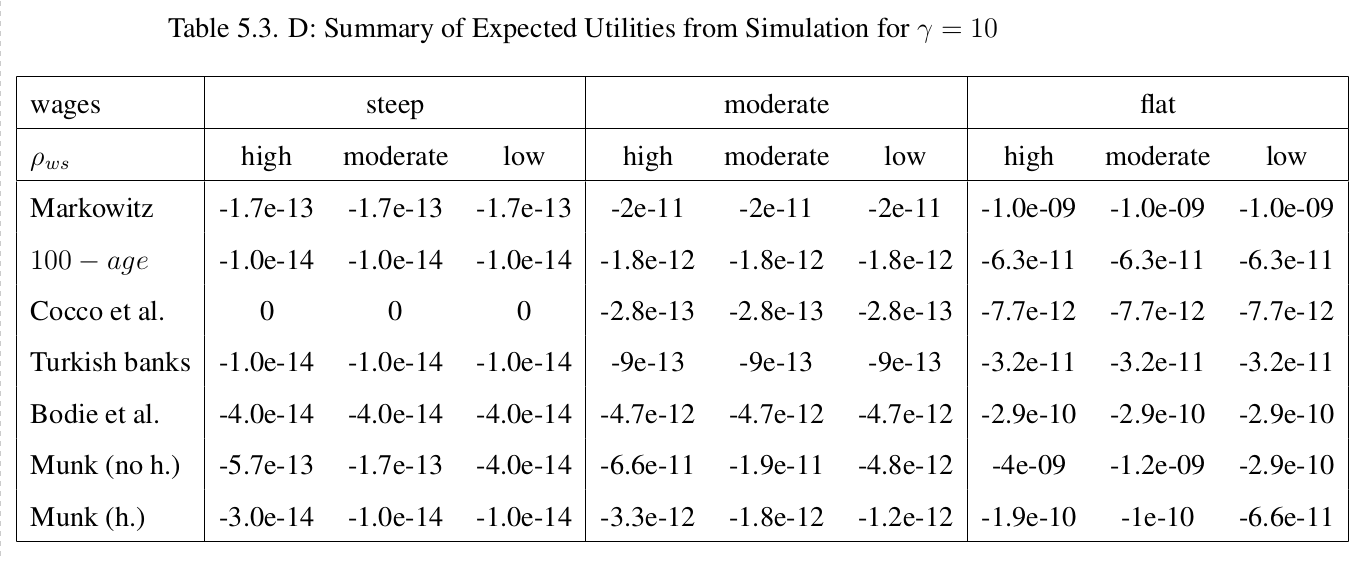
\includegraphics[scale=0.2]{figs/util10.png}
		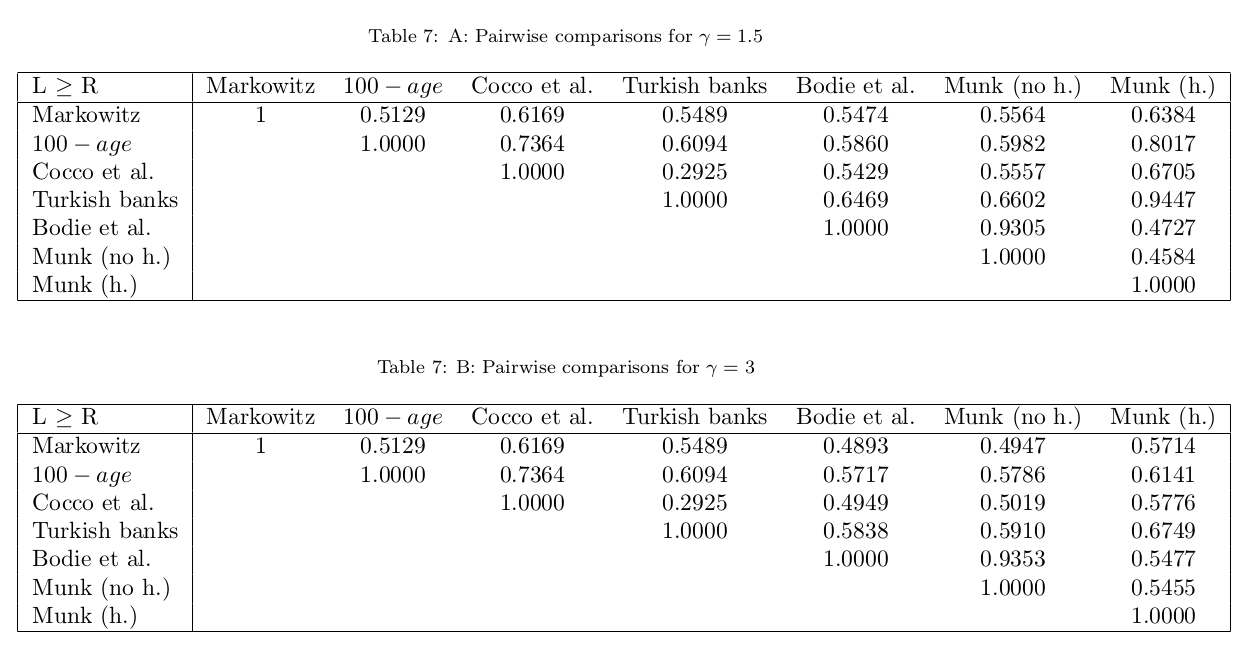
\includegraphics[scale=0.25]{figs/pair153.png}
		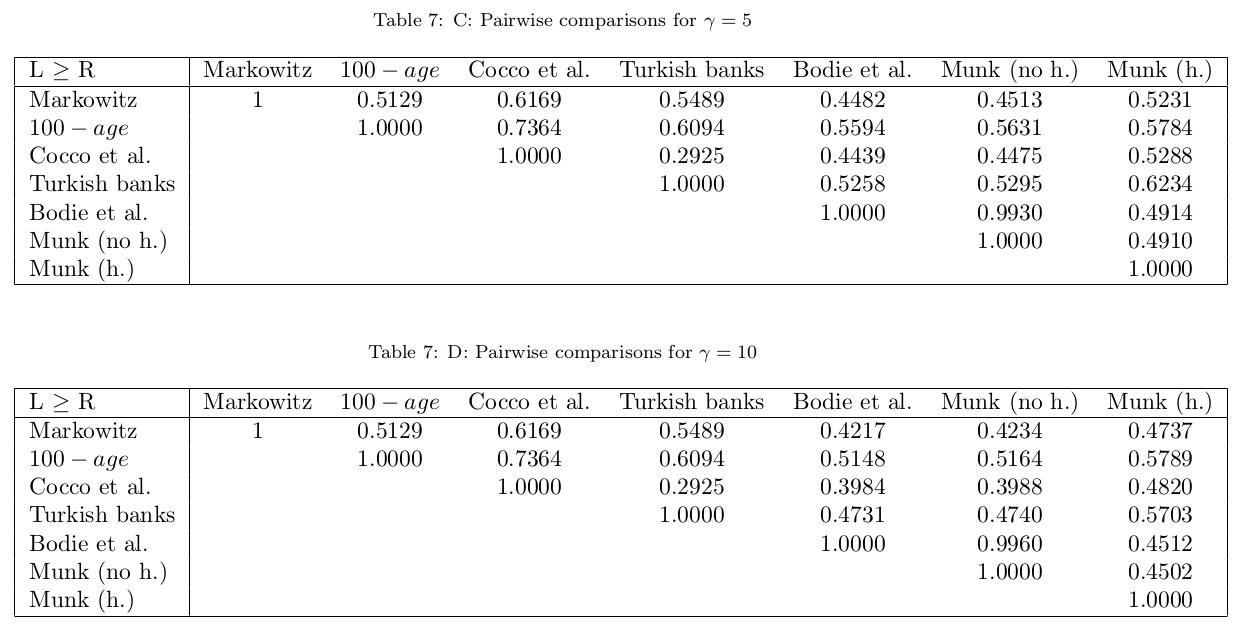
\includegraphics[scale=0.25]{figs/pair510.png}
	\end{figure}

\framebreak	

\framebreak

\framebreak

	\item After a lifetime of investing, the household accumulated various levels of wealth, summarized in the Table 5.1 of our thesis
	\item Looking at these total wealth levels, we can make early conclusions even before calculating utilities:
	\begin{itemize}
\item Cocco et al.'s $(200-2.5\cdot age)\%$ performs better, on average, than any other portfolio.
\item Even a naive life-cycle investment portfolio $(100-age)\%$ overperforms fixed-over-lifetime Markowitz.
\item All models perform better for higher risk aversion and worse for lower risk aversion.
\item Munk's solution performs worse for flat wages than for steep wages.
\item Munk's solution with housing is better than without housing when $\gamma > 1.5$.
\item When $\rho_{ws}=0$, Bodie's solution is almost equal to Munk's solution without housing, with the former performing slightly better than the latter.
\item Munk's solution with housing performs better for sectors with low stock-wage correlation, being a low-risk investment.
	\end{itemize}

	\item Expected utilities are summarized in Table 5.3 of our thesis.
  \end{itemize}
\end{frame}

\section{Conclusion}


\end{document}  
